\chapter{Exact Path Kernels Naturally Decompose Model Predictions}
\label{Chapter4a}

We can think about the previous paper establishing the exact path
kernel as an attempt to determine the necessary conditions for a
neural network to be expressed exactly by a kernel machine. The paper
also focused on using this kernel representation for uncertainty
quantification as an application. Although this is interesting from a
theory perspective, the applications are very limited and are a few
layers of abstraction away from providing any practical benefit to
modern machine-learning techniques. The purpose of the following paper
is to expand this theory and develop it towards applications that can
be directly useful to the field. In the process of generalizing and
applying the above method as a decomposition, it became obvious that
one modern machine-learning technique was implicitly relying on this
decomposition rather heavily : Out-of-Distribution (OOD)
Detection. The problem of identifying OOD data is orthogonal to the
adversarial problem. In some sense adversarial problems are difficult
because there do not exist practical metrics which can determine that
an adversarial example is not part of the natural data distribution
for a particular task. For OOD examples, data are generated by
distributions which are generally quite distinct from the distribution
of training data for an ML model. It can still be time-consuming or
difficult using statistical techniques to identify this data, so there
is a natural desire to use trained ML models to determine whether data
could be samples from the distributions they were trained on or
not. In many of the applications that follow

This Chapter includes a paper recently submitted to ICLR 2023. The
contents include a generalization of the representation from
~\ref{Chapter4} and two applications of this representation: First to
Out-Of-Distribution (OOD) detection, and the second to measuring
signal manifold dimension. These two applications begin to showcase
the advantages of path kernel ensemble representations of neural
networks. This was joint work primarily performed by Brian Bell,
Michael Geyer, where most of the theoretical work and mathematics was
derived and written by Brian Bell and the experimental work and
numerical results were produced by Michael Geyer. This particular
paper includes an extensive lit review (performed by Brian Bell)
analyzing some methods that have recently come to occupy the
cutting-edge of OOD detection algorithms. In the context of this
dissertation, this paper includes two important contributions, one is
a cleaner general definition of the representation from the previous
paper. The other is the decomposition of predictions by taking
gradients of this representation with respect to various spaces. This
second contribution allows the application of this theory to a class
of recent work and demonstrates the ability of this theoretical
foundation to inform practical applications at the cutting edge. 

%At the core of these contributions is the ability to compute the input sensitivities of training points on test predictions.

% Additionally, justifiable simplifying assumptions are provided which will allow this method to scale to cutting edge ML tasks.

% This manifold, which we call the observed manifold, is defined by the combination of data, model and training strategy.

\section{Introduction}

Out-of-distribution (OOD) detection for machine learning models is a new, quickly growing field important to both reliability and robustness~\citep{hendrycks2019, biggio2014, hendrycks2017, desilva2023, yang2021, filos2020autonomous}.
Recent results have empirically shown that parameter gradients are highly informative for OOD detection~\citep{behpour2023, djurisic2023extremely, huang2021}.
To our knowledge, this paper is the first to present theoretical justifications which explain the surprising effectiveness of parameter gradients for OOD detection.

In this paper, we unite empirical insights in cutting edge OOD with recent theoretical development in the representation of finite neural network models with tangent kernels~\citep{bell2023,chen2021equivalence,domingos2020}. 
Both of these bodies of work share approaches for decomposing model predictions in terms of parameter gradients. 
However, the Exact Path Kernel (EPK)~\citep{bell2023} provides not only rigorous theoretical foundation for the use of this method for OOD, but also naturally defines other decompositions which deepen and expand our understanding of model predictions. The application of this theory is directly connected to recent state of the art OOD detection methods.

In addition, this paper provides a connection between tangent kernel methods and dimension estimation.
At the core of this technique is the ability to extract individual training point sensitivities on test predictions.
This paper demonstrates a generalization (the gEPK) of the EPK from \citet{bell2023},  which can exactly measure the \emph{input gradient} $\nabla_{x_\text{train}}f(x_\text{test}, \theta_\text{trained})$.
It is shown that this quantity provides all necessary information for measuring the dimension of the \textit{signal manifold} \citet{srinivas2023} around a given test point.

\begin{figure}[t]
    \centering
    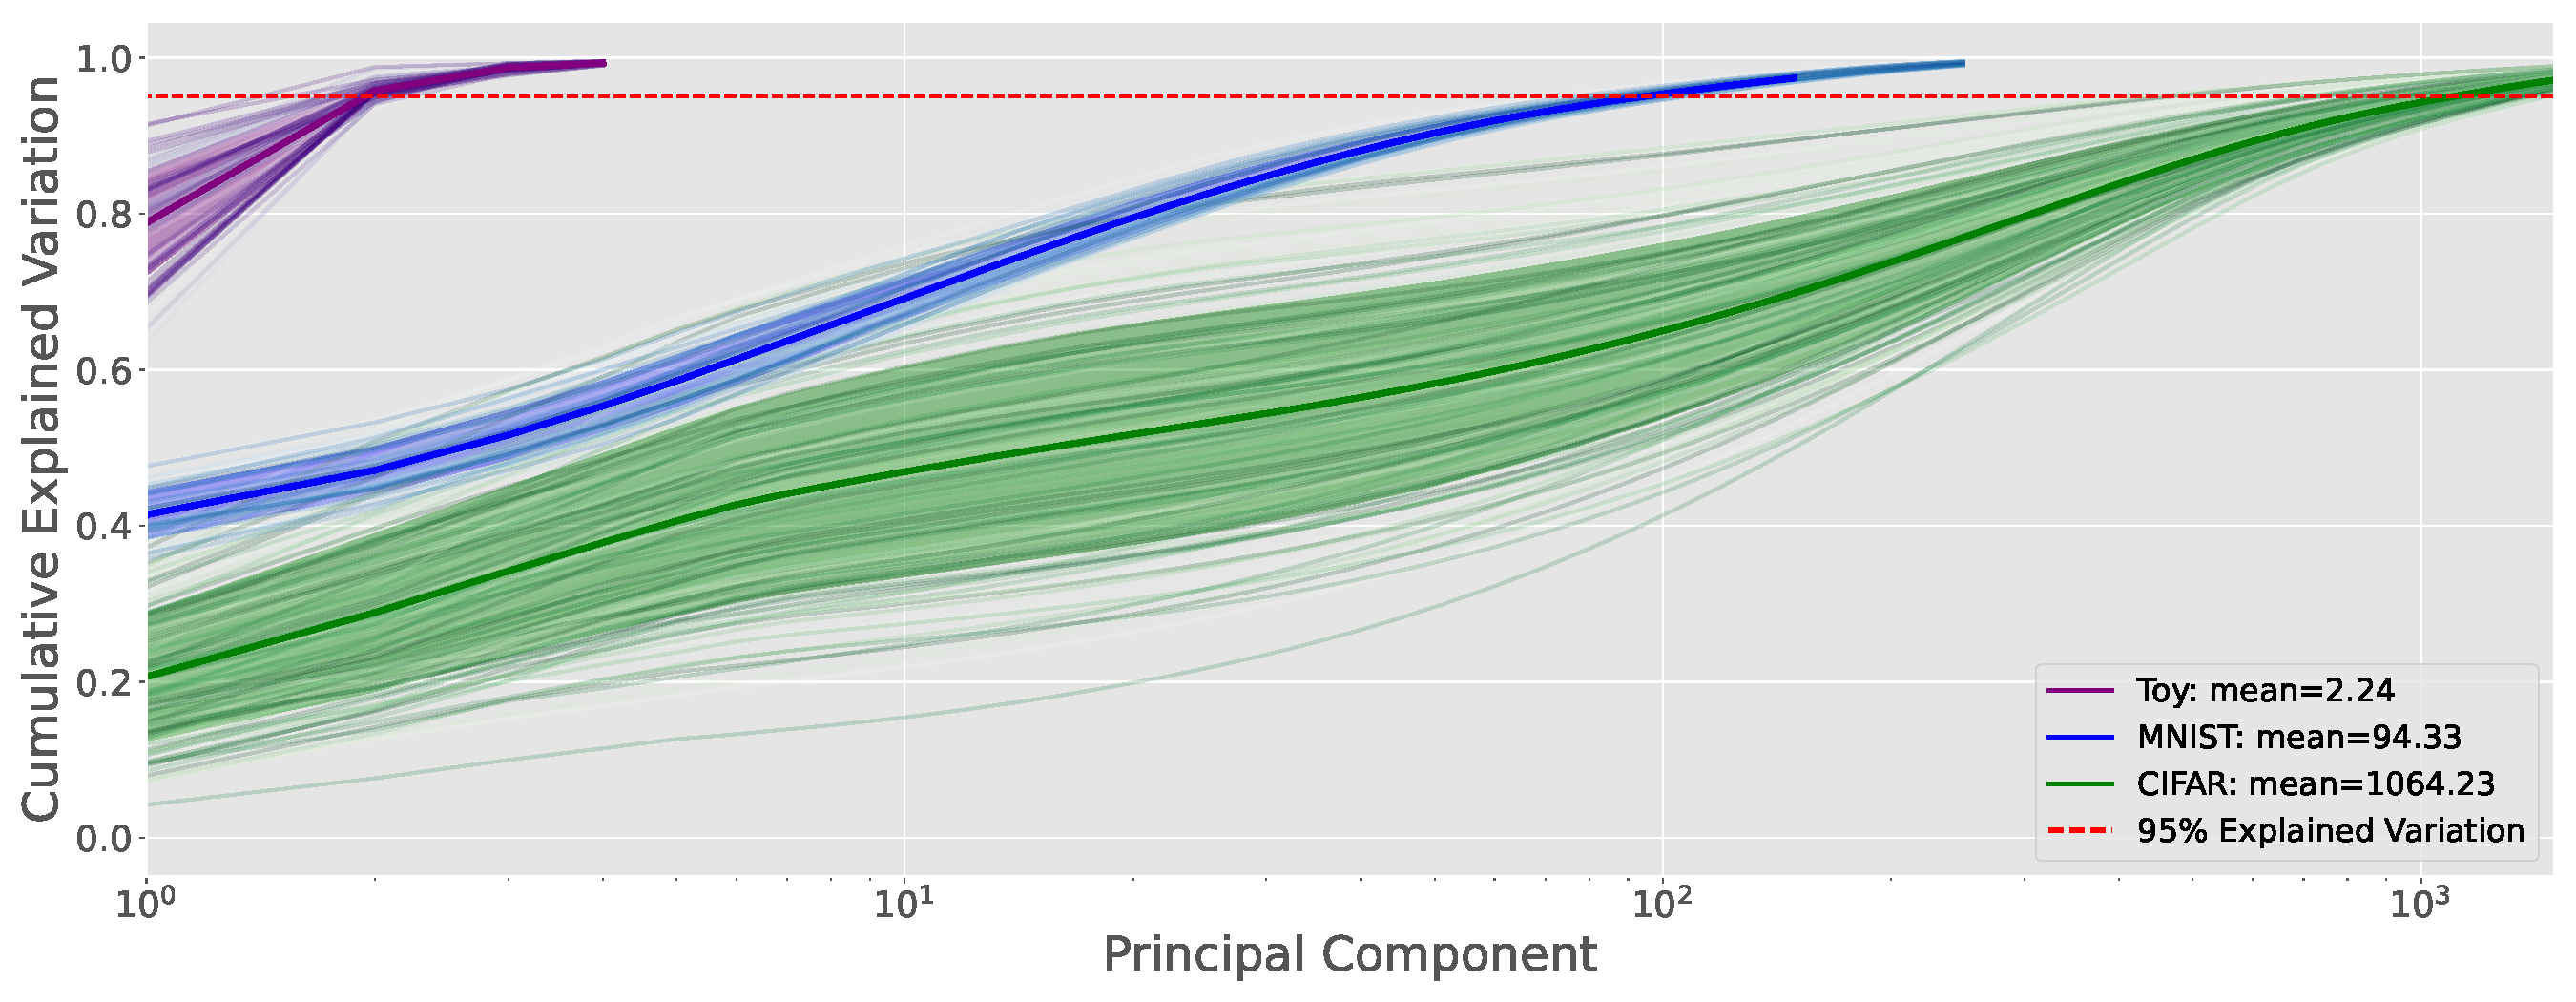
\includegraphics[width=0.9\textwidth]{c4a_figures/dimensionality_chords.pdf}
    % 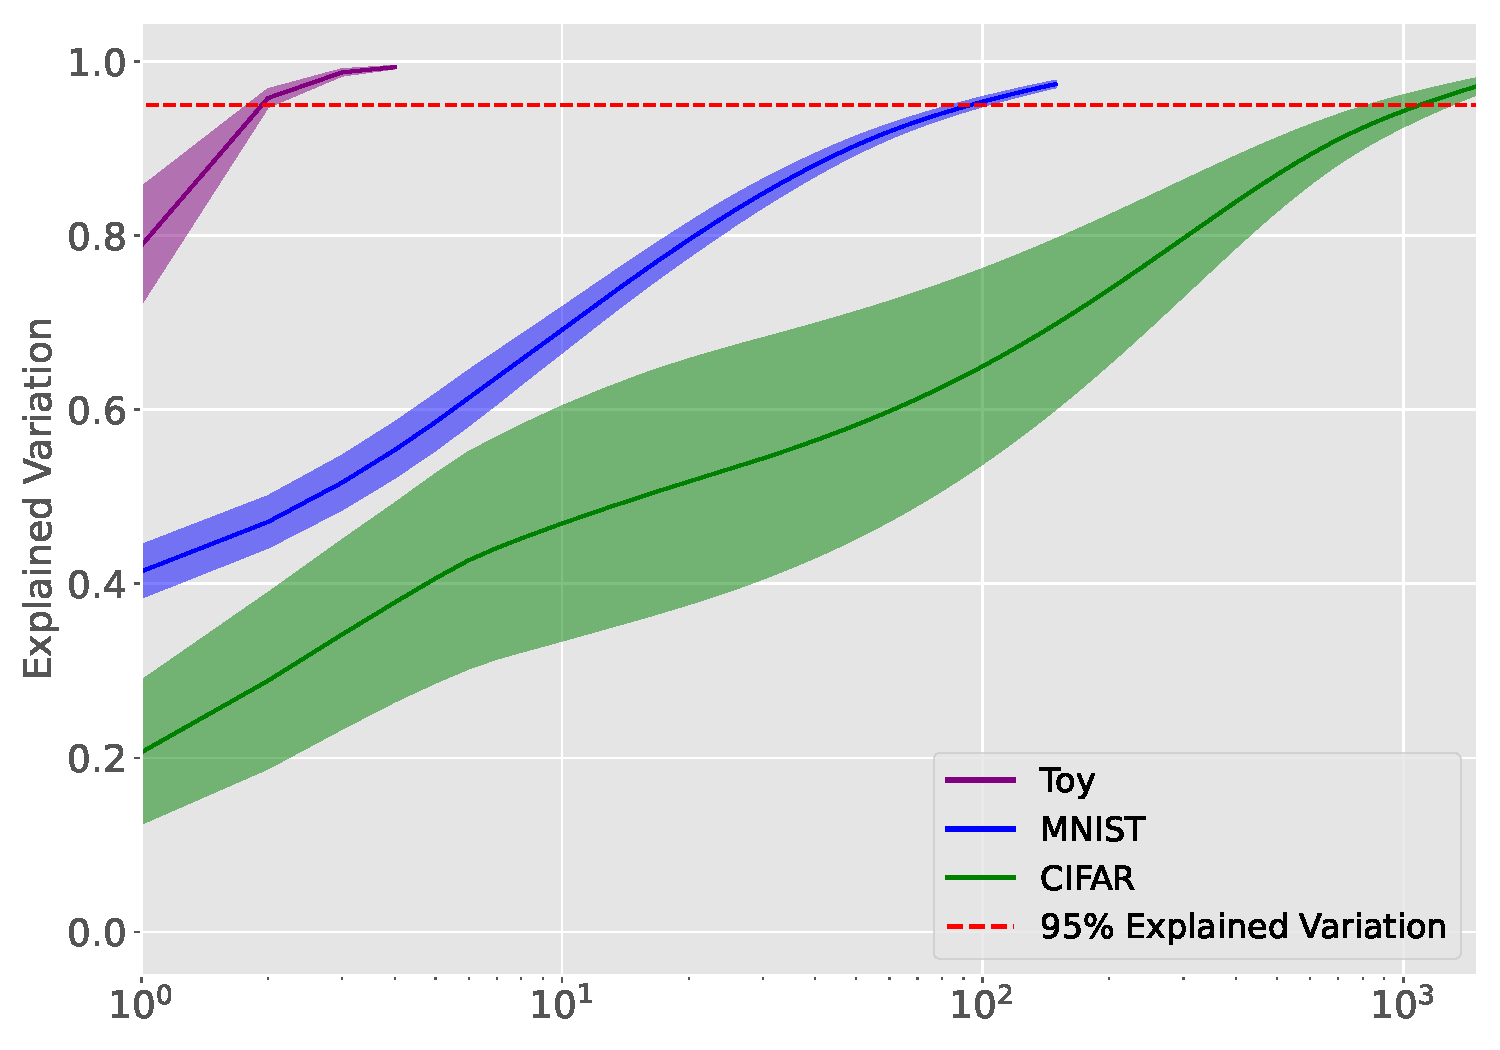
\includegraphics[width=0.45\textwidth]{c4a_figures/dimensionality_means.pdf}
    \caption{The gEPK naturally provides a measure of input dimension. This plot shows the CDF of the explained variation of training point sensitivities $\nabla_{x_\text{train}}f(x_\text{test}, \theta_\text{trained})$. Different datasets are color coded to show differences in signal dimension. Decomposing the input space in this way provides a view of the signal dimension around individual test points. For a toy problem (3 Gaussian distributions embedded in 100 dimensional space) the model only observes between 2 and 3 unique variations which contribute to 95\% of the information required for prediction. Meanwhile the dimension of the signal manifold observed by the model around MNIST and CIFAR test points is approximately 94 and 1064 respectively. }
    \label{fig:cdf}
\end{figure}
 
% This signal manifold, will be used to refer to the input subspace on which a model's predictions may vary.
% Until now, it has been impossible to exactly measure 
% This technique does not provide a measurement of intrinsic data dimension. 
% Many techniques which estimate data dimensions will for instance rely on the euclidean distance for nearest neighbor calculations, which can be unstable in high dimensional space.
% Instead, kernel methods provide a decomposition which measures the exact dimension of the input space which the model is able to observe.


In short, this work leverages the gEPK to:
\begin{itemize}
    \item Introduce a theoretical framework that provides a decomposition in terms of the previously proposed EPK. % explaining recent empirical methods in out-of-distribution detection.
    \item Generalize and explain the success of recent successful methods in OOD.
    \item Showcase OOD using natural gEPK based decomposition of model predictions in terms of parameter gradients.
    \item Measure exact input variations and signal manifold dimension around arbitrary test points.
    % \item Shed light on test time sensitivity of model predictions to training data using input gradients which are comparable across models the relationship between sensitivity tarnsfer and adversarial attack transfer.

\end{itemize}
The primary contributions of this paper are theoretical in nature: establishing the exact representation theorem in Section~\ref{sec:gepk} and writing several leading OOD detection methods in terms of this representation. The preliminary experimental results also support practical tasks of out-of-distribution (OOD) detection and estimating signal manifold dimension. 

\label{sec:input}

% Many prior works also attempt to answer the question of whether adversarial examples leave the data manifold \citet{gilmer2018adversarial, song2018pixeldefend}.
% This is again a difficult question to answer as the data manifold may be defined in many differing but valid ways.
% To simplify the problem, we will concern ourselves with two forms of manifold estimation.


% We provide a novel method of estimating the data manifold learned by a neural network.
% A clear definition for a comprehensive data manifold has been elusive thus far.
% The research community has 

% First, the manifold induced by the tangent space of a generative network, which we refer to as a \textit{generitive manifold}.
% The manifold induced by the directions in which the inputs may vary while not increasing the degrees of variation in weight gradients, which we refer to as the \textit{data-model manifold}.

% This second method of estimation is the primary contribution of this work, we demonstrate that


% Deep learning research is primarily driven by empirical results.

% Despite decades of research, many important questions, such as why certain architectures or regularization techniques improve performance have gone unanswered.
% One contributing reason for this is the complex and non-linear nature of neural networks.
% Analyzing these networks in order to develop mathematical frameworks of their behavior has proven extremely challenging.
% Another challenge is the high dimensionality of the data being consumed by these models.
% Many non-parametric techniques, such as clustering, fail in this high dimensional setting.
% In many areas of deep learning, theory has not caught up to practice.
% In this paper, we present a hypothesis which unifies several techniques that have empirically been shown to improve robustness of deep neural networks.



% \section{Related Work}

% \subsection{Model Gradients}
% The input gradients of discriminative models have been studied as a method of model explainability.
% The magnitude of these input gradients is often used as a fundamental feature attribution technique \citet{baehrens2010explain, simonyan2013deep}.
% Recent work demonstrates that many saliency methods fail basic sanity checks which should be expected out of explanation methods \citep{adebayo2018sanity, kindermans2019reliability}.
% The majority of these methods are build on careful measurement of input gradients.
% \citet{shah2021input} show that input gradient magnitude is not a consistent measure of feature attribution for standard models.
% In contrast, they show evidence that the input gradients of robust models are useful for feature attribution.
% This property of robust models is still not fully understood, however some hypotheses attempt to explain the relationship between robustness and PAG.
% The dimpled manifold hypothesis \citep{shamir2021dimpled} claims that images lie on some low-dimensional manifold, and model decision boundaries 'dimple' around individual data points.
% There also exists the hypothesis that there exist 'brittle' and 'robust' features in natural data and adversarial training forces a model to only focus on robust features \citet{ilyas2019adversarial, tsipras2019robustness}.

% \subsection{OOD}

\section{Related Work}
While there has been a significant amount of recent work studying the Neural Tangent Kernel (NTK)~\citep{jacot2018neural}, there is still relatively little work exploring its exact counterpart, the path kernels~\citep{bell2023, chen2021equivalence, domingos2020}. While these other works are focused on the precise equivalence between artificial neural networks and SVMs or Kernel machines, this equivalence requires significant restrictions placed on the loss function and model used for a task. This paper seeks to take advantage of this exact representation style without imposing such strict requirements. To the best of our knowledge, this is the first work exploring this loosened equivalence. 


There are several schools of thought, whether OOD data can be learned~\citep{huang2021scaling, mohseni2020, he2015, pillai2013classification, fumera2002}, which part of a model should be interrogated in order to identify OOD examples~\citep{liu2020, lin2021}, whether it is a purely statistical question~\citep{lee2018}, or whether it can simply be solved with more data~\citep{chen2021atom, de_silva_value_2023}. The best performing recent approaches have all used relatively simple modifications of model activation or model gradients \citep{djurisic2023extremely, xu2023vra, sun2022, sun2021}. The first methods we explore (see Section~\ref{sec:ood} relates to the use of model gradients to construct statistics which separate in-distribution (ID) examples from OOD examples. This is fundamentally a geometric approach which should be comparable with the method proposed by \citet{sun2022deep}~\citep{gillette2022data} The first prominent method of this type was proposed by~\citet{liang2018}. ODIN is still a notable method in this space, and has been followed by many more gradient based approaches~\citep{behpour2023, huang2021gradients} and has caused some confusion about why these methods work so well~\citep{igoe2022}

Much recent work has been devoted to measurement of dimension for the subspace in which the input data distribution live for machine-learning tasks. We will partition this work into works trying to understand this intrinsic data dimension in model agnostic ways~\citep{gillette2022data, yousefzadeh2021deep, kaufman_data_2023, gilmer2018, gong2019, glielmo2022, facco2018, Levina_Bickel_2004} and works trying to understand or extract model's understanding of this subspace~\citep{dominguez-olmedo_data_2023, Ansuini_Laio_Macke_Zoccolan_2019, talwalker2008, Costa_Hero_2004b, giryes2014, Zheng_He_Qiu_Wipf_2022}. This paper proposes a new method which bears more similarity to the latter. We argue that this approach is more relevant for studying ANNs since they discover their own metric spaces. This paper, additionally, provides tools for exact measurement of the signal manifold around a given test point. Understanding signal manifolds is both useful in practice for more efficient low rank models~\citep{yang2020, swaminathan2020}, and also for uncertainty quantification and robustness~\citep{Costa_Hero_2004a, wang2021, khoury2018, srinivas2023, song2018pixeldefend, snoek2019}. Along with OOD, uncertainty quantification is increasingly relying on gradients as demonstrated by~\citet{lee2020} and this paper seeks to also support these methods. 

\section{Theoretical Justification : Generalized Exact Path Kernel}
\label{sec:gepk}
The theoretical foundation of this paper generalizes a recent exact path kernel representation result from~\citet{bell2023}. 
We will reuse the structure of the Exact Path Kernel (EPK) without relying on the reduction to a single kernel across training steps. For classification models trained with cross-entropy loss~\citet{bell2023} showed that the summation over training steps defines a kernel.
In order to increase generality, we do not assume the cross-entropy loss, resulting in a representation which is not strictly a kernel.
The function, $\varphi_{s,t}(x)$, in the EPK sum defines a bilinear subspace, the properties of which we will study in detail.
This representation however, will allow exact and careful decomposition of model predictions according to both input gradients and parameter gradients without the strict requirements of the EPK.

\begin{restatable}[Generalized Exact Path Kernel (gEPK)]{theorem}{ekr}
\label{thm:ekr}
Suppose $f(\cdot; \theta)$ is a differentiable parametric model with parameters $\theta \in \mathbb{R}^M$ and $L$ is a loss function. Furthermore, suppose that $f$ has been trained by a series $\{\theta_s\}_{s=0}^S$ of discrete steps composed from a sum of loss gradients for the training set $ \sum_{i}^N \varepsilon \nabla_\theta L(f(x_i), y_i)$ on $N$ training data $X_T$ starting from $\theta_0$. Then for an arbitrary test point $x$, the trained model prediction $f(x; \theta_S)$ can be written:
\begin{equation}
f(x; \theta_S) = f(x; \theta_0) + \sum_{i=1}^N \sum_{s=1}^S \varepsilon \left(\int_0^1 \varphi_{s,t}(x) dt\right) \dfrac{dL(f(x_i, \theta_s), y_i)}{d \hat y_{\theta_s(0)}} \left(\varphi_{s, 0}(x_i)\right)
\label{exact}
\end{equation}
% Where
\begin{align}
    \varphi_{s,t}(x) &\equiv \nabla_\theta f(x; \theta_s(t)), \\
    \theta_s(t) &\equiv \theta_s(0) + t(\theta_{s+1}(0)-\theta_s(0)), \text{ and}\\
    \hat y_{\theta_s(0)} &\equiv f(x; \theta_s(0)).
\end{align}
\end{restatable}
% \subsection{The EPK gives an Exact Representation}
% \label{proof:eker}
% \eker*
\begin{proof}
Guided by the proof for Theorem 6 from~\citet{bell2023}, let $\theta$ and $f(\cdot; \theta)$ satisfy the conditions of Theorem~\ref{thm:ekr}, and $x$ be an arbitrary test point. We will measure the change in prediction during one training step from $\hat y_s = f(x; \theta_s)$ to $\hat y_{s+1} = f(x; \theta_{s+1})$ according to its differential along the interpolation from $\theta_s$ to $\theta_{s+1}$. Since we are training using gradient descent, we can write $\theta_{s+1} \equiv \theta_s + \dfrac{d \theta_s(t)}{dt} $. We derive a linear interpolate connecting these states:
\begin{align}
    \dfrac{d \theta_s(t)}{dt} &= (\theta_{s+1} - \theta_s)\\   
    \int \dfrac{d \theta_s(t)}{dt} dt &= \int (\theta_{s+1} - \theta_s)dt\\
    \theta_s(t) &= \theta_s + t(\theta_{s+1} - \theta_s)
\end{align}
Since $f$ is being trained using a sum of gradients weighted by a constant scalar $\varepsilon$, we can write:
\begin{align}
    \dfrac{d \theta_s(t)}{dt} &= -\varepsilon  \nabla_w  L(f(X_T; \theta_s(0)), y_i) = -\sum_{i=1}^N \varepsilon \sum_{j = 1}^{M}   \dfrac{\partial L(f(x_i; \theta_s(0)),  y_i)}{\partial \theta^j} \label{eq10}
\end{align}
Applying chain rule and the above substitution, we can write the change in the prediction as 
\begin{align}
    \dfrac{d \hat y}{dt} = \dfrac{d f(x; \theta_s(t))}{dt} &= \sum_{j = 1}^{M} \dfrac{d f}{\partial \theta^j} \dfrac{\partial \theta^j}{dt} = \sum_{j = 1}^{M} \dfrac{d f(x; \theta_s(t))}{\partial \theta^j} \left(-\varepsilon  \dfrac{\partial L(f(X_T, \theta_s(0)),  Y_T)}{\partial \theta^j}\right)\\
&= \sum_{j = 1}^{M} \dfrac{d f(x; \theta_s(t))}{\partial \theta^j} \left(- \sum_{i = 1}^{N}\varepsilon\dfrac{d L(f(x_i; \theta_s(0)),  y_i)}{d f(x_i; \theta_s(0))}\dfrac{\partial  f(x_i; \theta_s(0))}{\partial \theta^j}\right)\\
&= - \sum_{i = 1}^{N} \varepsilon \nabla_w f(x; \theta_s(t)) \dfrac{d L(f(x_i; \theta_s(0)),  y_i)}{d f(x_i; \theta_s(0))}  \cdot \nabla_w f(x_i; \theta_s(0))
\end{align}
Using the fundamental theorem of calculus, we can compute the change in the model's output over step $s$,
\begin{align}
    y_{s+1} - y_s &= \int_0^1 -\sum_{i = 1}^{N} \varepsilon\dfrac{d L(f(x_i; \theta_s(0)),  y_i)}{d f(x_i; \theta_s(0))}  \nabla_w f(x; \theta_s(t)) \cdot \nabla_w f(x_i; \theta_s(0))dt\\
 &=  - \sum_{i = 1}^{N} \varepsilon\left(\int_0^1\nabla_w f(x; \theta_s(t))dt\right) \dfrac{d L(f(x_i; \theta_s(0)),  y_i)}{d f(x_i; \theta_s(0))}   \cdot \nabla_w f(x_i; \theta_s(0))
\end{align}
For all $N$ training steps, we have
\begin{align}
y_N &= f(x; \theta_0) + \sum_{s=1}^N y_{s+1} - y_s \\
&= f(x; \theta_0) - \sum_{s = 1}^N \sum_{i = 1}^{N} \varepsilon\left(\int_0^1\nabla_w f(x; \theta_s(t))dt\right) \dfrac{d L(f(x_i; \theta_s(0)),  y_i)}{d f(x_i; \theta_s(0))}   \cdot \nabla_w f(x_i; \theta_s(0))
\end{align}
\end{proof}
    
% \textbf{Remark 1:} \\
\textbf{Remark 1:} We note that the training data need not remain fixed for each step of training, the equivalence holds with a different set of training data used at each step, e.g. as in SGD.  \\
\textbf{Remark 2:} This representation holds true for any contiguous subset of a gradient based model, e.g. when applied to only the middle layers of an ANN or only to the final layer. This is since each contiguous subset of an ANN can be treated as an ANN in its own right with the activations of the preceding layer as its inputs and its activations as its outputs. In this case, the training data consisting of previous layer activations may vary as the model evolves. % We will assume that the data we are learning has structure which is locally linear.
% We will assume the signal manifold is continuous and fully connected. % improve wording of terms here
% % All points within the dataset are considered to be on the signal manifold, and for any pair of points $x_i, x_j \in \mathcal{D}$ there exists an interpolation path for which all intermediate points are on the signal manifold.
% The Exact Path Kernel representation of a neural network represents the training set as gradient vectors in weight space.
% The inner product of these gradient vectors with a similarly transformed test vector allows a measure of distance between training and testing data.

\section{OOD is enabled by Parameter Gradients}
\label{sec:ood}
\begin{figure}[h]
\begin{center}
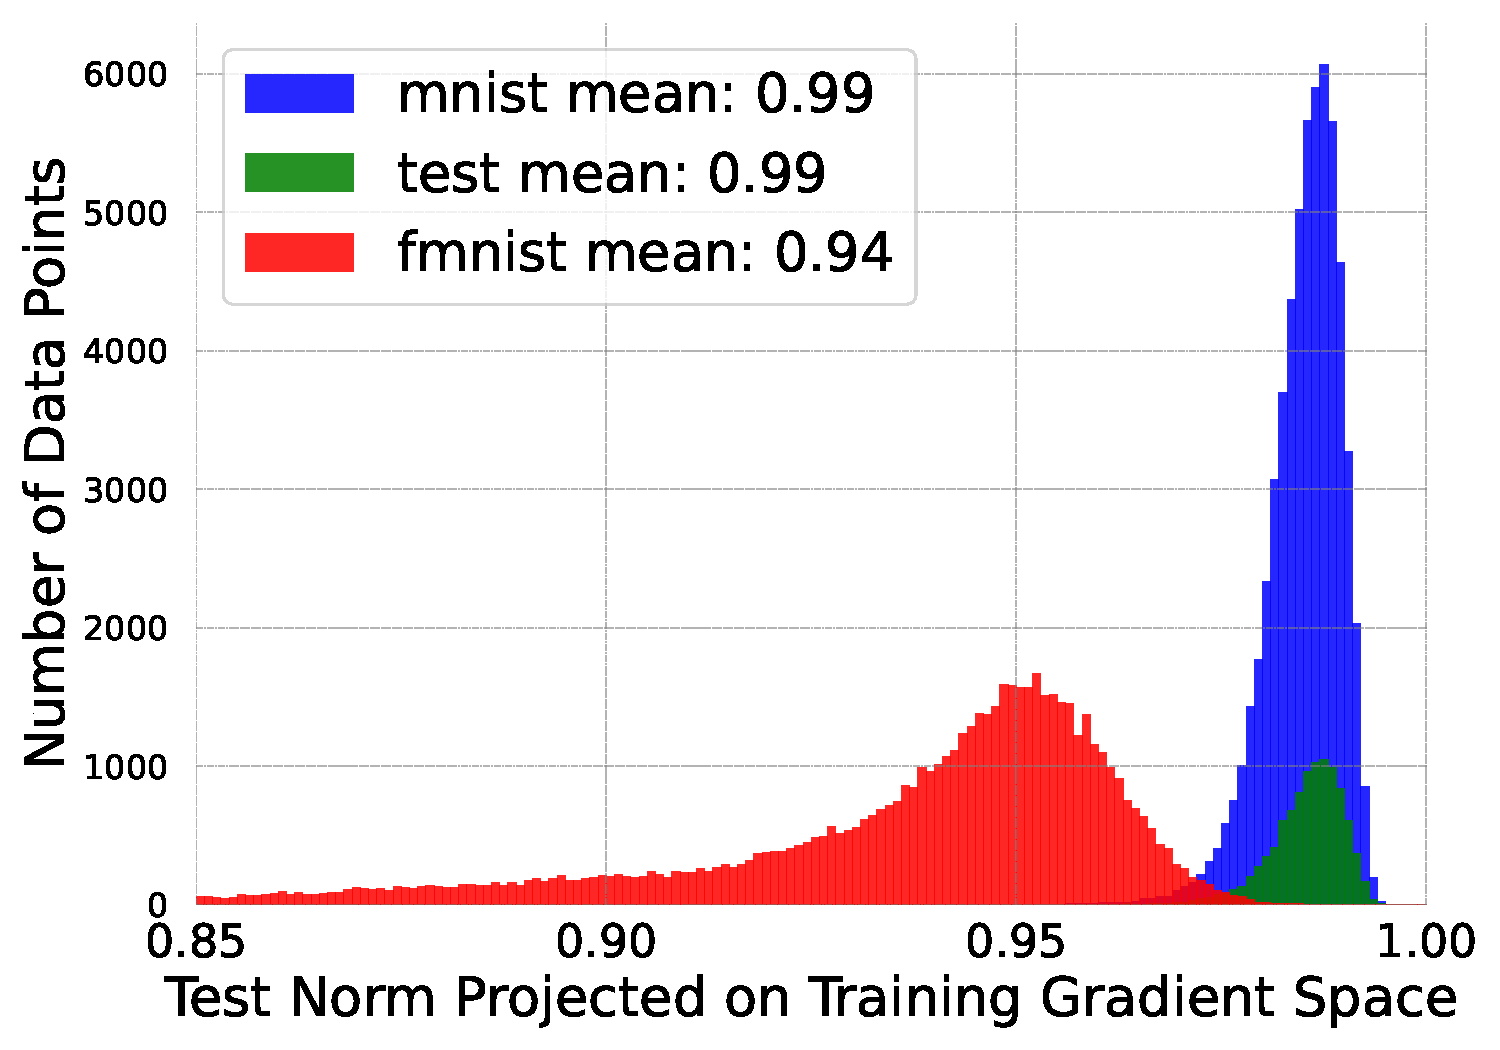
\includegraphics[width=0.45\textwidth]{c4a_figures/grad_alignment_hist.pdf}
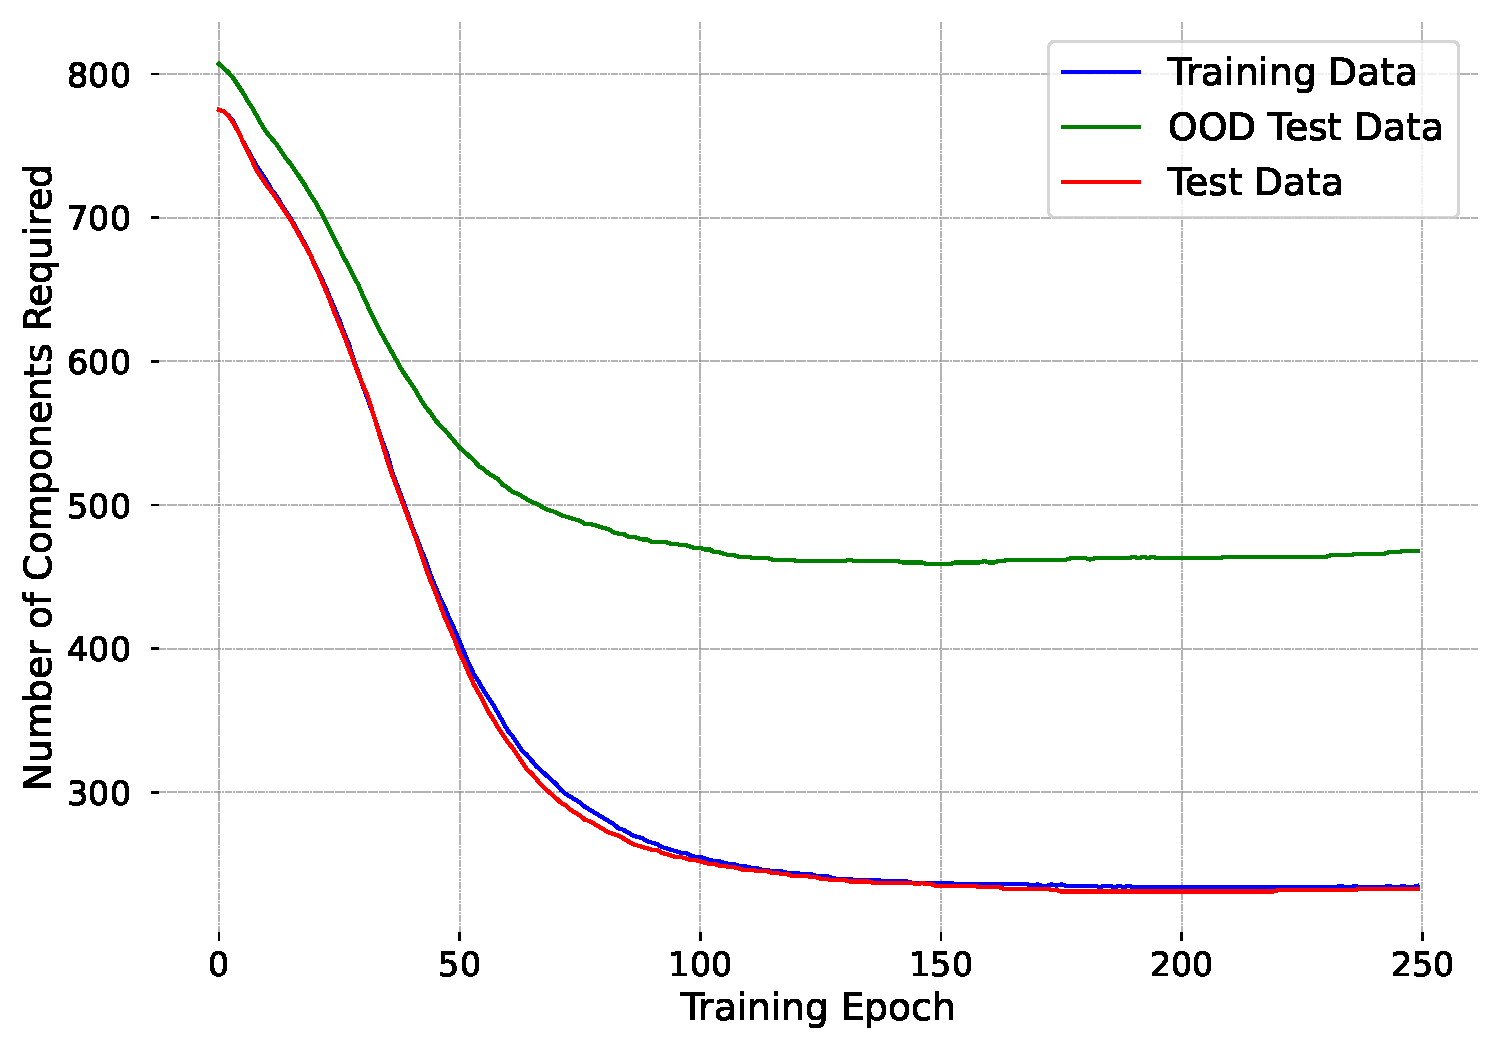
\includegraphics[width=0.45\textwidth]{c4a_figures/ood_noise.pdf}
%\framebox[4.0in]{$\;$}
% \fbox{\rule[-.5cm]{0cm}{4cm} \rule[-.5cm]{4cm}{0cm}}
\end{center}
\caption{OOD detection using difference in training vs. test gradients. As the purpose of this paper is not to develop state of the art OOD detection methods, a comparison with recent benchmarks is not provided. Instead, a proof of concept that the gEPK can perform OOD detection is given. Left histogram shows norms of vectors projected onto the gradient weight space defined by the gEPK on MNIST and FMNIST. Right plot shows the number of components required to explain 95\% variation in weight space across training for a toy problem (three Gaussian distributions embedded in 100 dimensions). }
\label{fig:ood}
\end{figure}
One natural application of the gEPK is the separation of predictions into vectors corresponding with the test gradient $\varphi_{s,t}(x)$ for a given test point $x$ and each training vector  weighted by its loss gradient $\dfrac{dL(\hat y_i, y_i)}{d\hat y_i} \varphi_{s, 0}(x_i)$. While the test vector depends on the choice of test point $x$, the subspace of training gradient vectors is fixed. By the linear nature of this inner product, it is clear that no variation in test data which is orthogonal to the training vector space can be reflected in a model's prediction. We can say that 
\begin{align}
    \left\{\dfrac{dL(\hat y_i, y_i)}{d\hat y_i} \varphi_{s, 0}(x_i); i \in \{1,...,N\}, s \in \{1,...,S\}\right\}
\end{align}
spans the subspace in which all model predictions can vary. Empirically, we compute the SVD of these training parameter gradients summing over classes in Fig.~\ref{fig:rank}. This shows that the space does most of its variation is within only a few dimensions for each test point. Additionally, this corresponds with the well-established notion that the latent dimension of data is much smaller than its ambient dimension. It is by analyzing spectra of this subspace that we may accomplish out-of-distribution (OOD) detection, and, in fact, we will demonstrate that this is how most cutting-edge OOD methods discriminate in practice. 

\subsection{Expressing Prior OOD Methods with the gEPK}

 We will now establish that most gradient based methods for OOD and some methods which do not explicitly rely on gradients can be written as projections onto subsets of this span. 



% \subsection{GradNorm}
\textbf{GradNorm}
The first well-known method to apply gradient information for OOD is  ODIN: Out-of-DIstribution detector for Neural Networks  \citet{liang2018}. This method, inspired by adversarial attacks, perturbs inputs by applying perturbations calculated from input gradients. The method then relies on the difference in these perturbations for in-distribution versus out-of-distribution examples to separate these in practice. This method directly inspired~\citet{huang2021} to create GradNorm. This method which occupied the cutting edge in 2021 computes the gradient of Kullback–Leibler divergence with respect to model parameters so that:
% \begin{align}
%     \dfrac{\partial D_{KL}(u||\text{softmax}(f(x)))}{d\theta} &= \dfrac{1}{C} \sum_i^C \dfrac{\partial L_{CE}(f(x), i)}{d\theta}
%     \end{align}
    % We can rewrite this in notation more consistent with the gEPK
\begin{align}
    \dfrac{1}{C} \sum_i^C \dfrac{\partial L_{CE}(f(x; \theta), i)}{\partial\hat y}\nabla_\theta f(x; \theta)
\end{align}
This looks like the left side of the inner product from the gEPK, however the scaling factor, $\dfrac{\partial L_{CE}(f(x; \theta), i)}{d\hat y}$, does not match. In fact, this approach is averaging across the parameter gradients of this test point with respect to each of its class outputs, which we can see is only a related subset of the full basis used by the model for predictions. This explains improvements made in later methods that are using a more full basis. Another similar method, ExGrad~\citep{igoe2022}, has been proposed which experiments with different similar decompositions and raises some questions about what is special about gradients in OOD -- we hope our result sheds some light on these questions. Another comparable method proposed by ~\citet{sun2022deep} may also be equivalent through the connection we establish below in Section~\ref{sec:input} between this decomposition and input gradients which may relate with mapping data manifolds in the Voronoi/Delaunay~\citep{gillette2022data} sense. 

\textbf{ReAct, DICE, ASH, and VRA}
Along with other recent work~\citep{sun2021, sun2022, xu2023vra}, some of the cutting edge for OOD as of early 2023 involves activation truncation techniques like that neatly described by~\citet{djurisic2023extremely}. Given a model, $f(x; \theta) = f^{\text{extract}}(\cdot; \theta_{\text{extract}}) \circ f^{\text{represent}}(\cdot; \theta_{\text{represent}}) \circ f^{\text{classify}}(\cdot; \theta_{\text{classify}})$, and an input, $x$, a prediction, $f(x, \theta)$, is computed forward through the network. This yields a vector of activations, $A(x, \theta_{\text{represent}})$, in the representation layer of the network. This representation is then pruned down to the $p^{\text{th}}$ percentile by setting any activations below that percentile to zero. ~\citet{djurisic2023extremely} mention that ASH does not depend on statistics from the training data, however by chain rule, high activations will correspond with high parameter gradients. That means that this truncation is picking a representation for which $\left\langle \nabla_\theta f(x, \theta_{\text{represent}}), \dfrac{dL(\hat y(x_i), y_i)}{d\hat y} \nabla_\theta f(x_i, \theta_{\text{represent}}) \right\rangle$ is high for many training data, $x_i$. This is effectively a projection onto the parameter tangent space of the training data with the highest variation. This may explain some part of the performance advantage of these method. 

\begin{figure}[t]
    \centering
    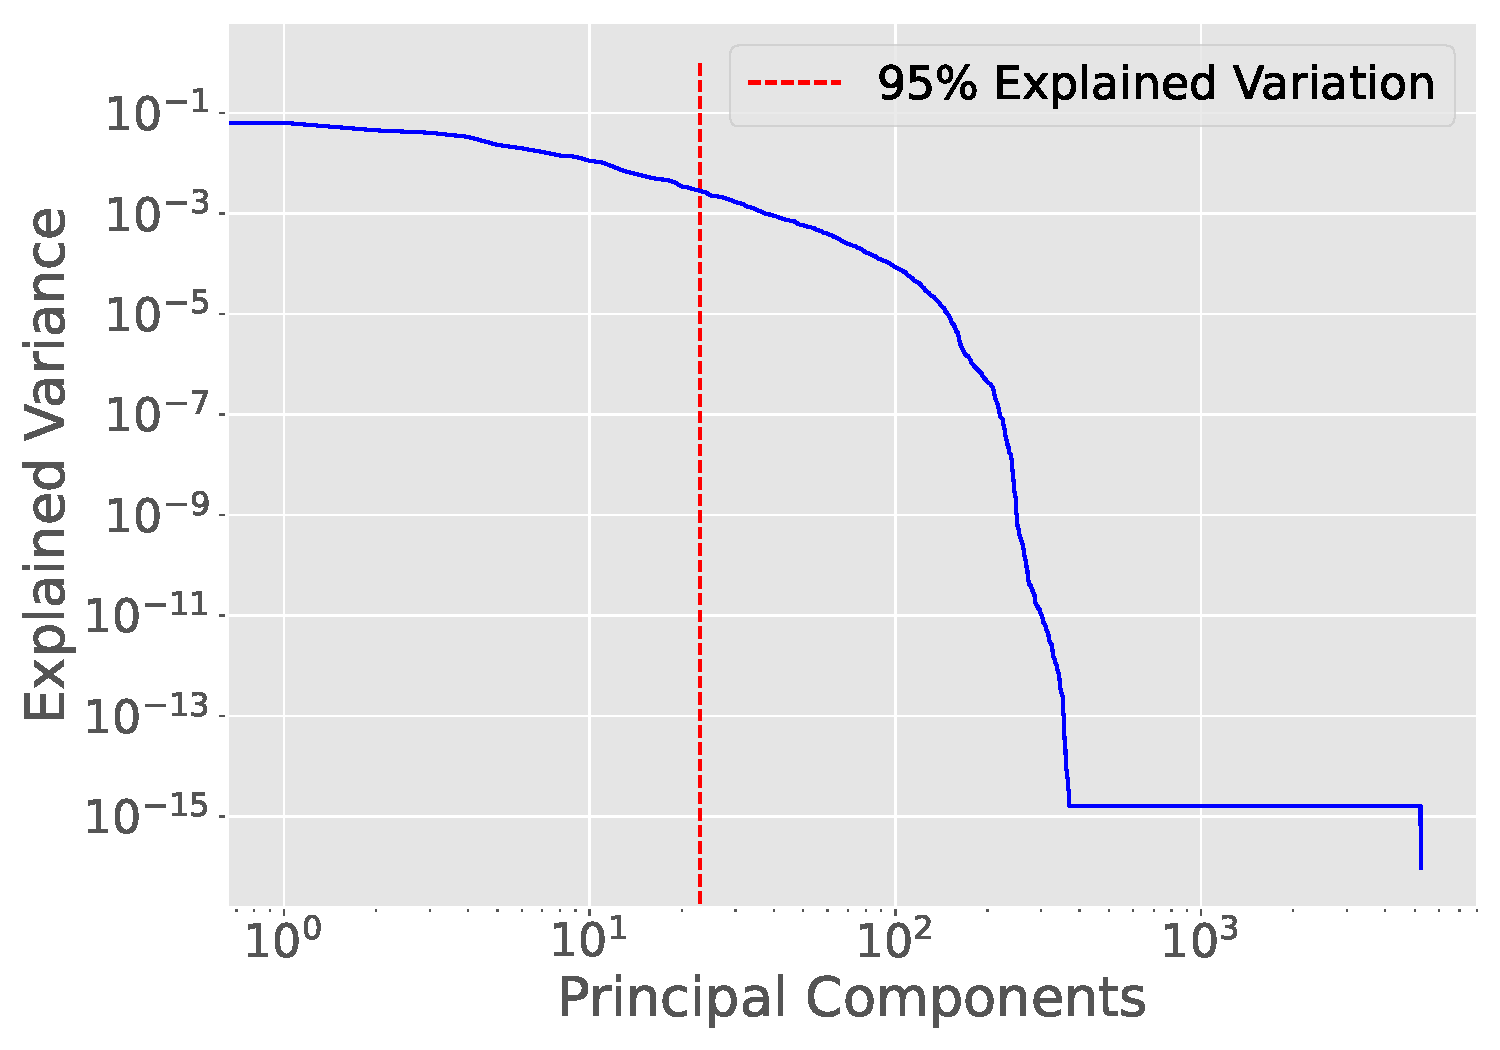
\includegraphics[width=0.45\textwidth]{c4a_figures/explained_variance_ratio.pdf}
    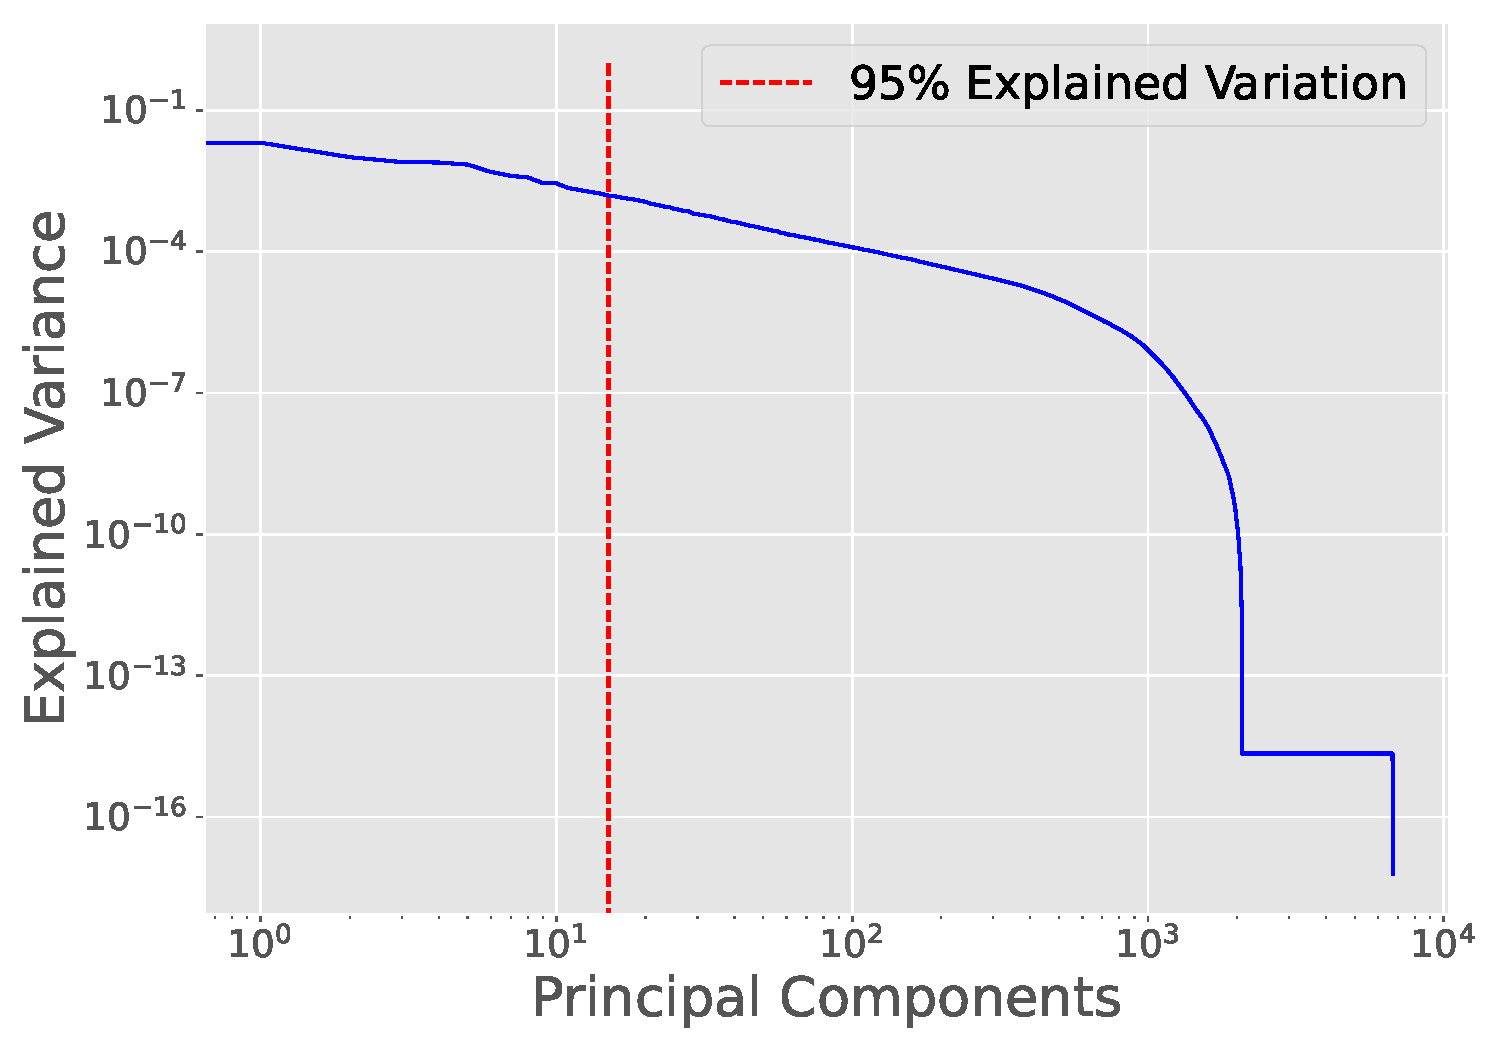
\includegraphics[width=0.45\textwidth]{c4a_figures/explained_variance_ratio_cifar.pdf}
    \caption{Explained Variance Ratio of parameter gradients. Left: MNIST, Right: CIFAR. 95\% of variation can be explained with a relatively low number of components in both cases.}
    \label{fig:rank}
\end{figure}

\textbf{GradOrth}~\citet{behpour2023} explicitly create a reference basis from parameter gradients on training data for comparison. They do this for only the last layer of a network with mean squared error (MSE) loss, allowing a nicely abbreviated expression for the gradient:
\begin{align}
    \nabla_\theta L(x, y) &= (\theta x - y)x^T = \Omega x^T
\end{align}
Treating $\Omega$ as an error vector, they prove that all variation of the output must be within the span of the $x^T$ over the training set. They then pick a small subset of the training data and record its activations $R^L_{ID} = [x_1, x_2, ..., x_n]$ over which they compute the SVD, $U^L_{ID} \Sigma^L_{ID} (V^L_{ID})^T = R^L_{ID}$. This representation is then truncated to $k$ principal components according to a threshold $\epsilon_{\text{th}}$ such that 
\begin{align}
\left\| U^L_{ID} \Sigma^L_{ID, k} (V^L_{ID})^T\right\|^2_F &\geq \epsilon_\text{th} \|R^L_ID\|^2_F.
\end{align}
This basis $S^L = (U^L_ID)_k$ is now treated as the reference space onto which test points' final layer gradients can be projected. Their score is 
\begin{align}
    O(x) = (\nabla_{\theta_L} \mathcal{L}(f(x, \theta_L), y))S^L(S^L)^T
\end{align}
We note that this formulation requires a label $y$ for each of the data being tested for inclusion in the data distribution. Despite this drawback, the performance presented by \citet{behpour2023} is impressive.~\citet{behpour2023} also present a brief proof that gradient updates for the final layer parameters $\theta_L$ for an optimization step defined by a batch of training data must be within the span of the final layer activation for that batch. While this is true, it may greatly underestimate the true rank of the data and also may not necessarily map the correct magnitude of variations along each of the basis directions. 


\subsection{gEPK for OOD}
The gEPK provides a more general spanning result immediately. Indeed, the network's prediction can only be influenced by $\{\varphi_{s, 0}(x_i)\}$ for the training data batched for each step, $s$. 
Loss in the gEPK only appears for the training points. This means that $\varphi_{s, t}(x) = \nabla_\theta f(x; \theta_s(t))$ can be computed for any test point without need for a label. Then all parameter gradients must live in:
\begin{align}
\text{span}\left(\left\{\dfrac{dL(\hat y_i, y_i)}{d\hat y_i} \varphi_{s, 0}(x_i) : x_i \in X_T , 0 \leq s \leq S\right\} \right). 
\end{align}

We can see that most, if not all, of the above methods can be represented by some set of averaging assumptions on the representation provided by the gEPK. We test the ability of the gEPK to perform OOD detection by direct projection onto the full parameter gradient space spanned by its training parameter gradients using a sum over the class outputs in Fig.~\ref{fig:ood}. Indeed, the gEPK helps explain the high performance of gradient based methods due to the implicit inclusion of the training parameter space in model predictions. This serves to illuminate the otherwise confusing discrepancy raised by~\citet{igoe2022}. 

\begin{figure}[t]
\begin{center}
\begin{tikzpicture}
\node [anchor=north, scale=1.0] (note) at (3.48,9.2) {Testing Point};
\node [anchor=west, rotate=90, scale=1.0] (note) at (0.20,1.8) {Training Point};
\node [anchor=north, scale=0.85] (water) at (2.5,8.7) { Model A};
\node [anchor=north, scale=0.85] (water) at (4.45,8.7) { Model B};
\node [anchor=south] (silly) at (0, -0.5) {};
\node [anchor=south] (silly) at (6, -0.5) {};
%\node [anchor=north] (water) at (1,1) {\Large Model B};
\begin{scope}[xshift=0.5cm]
    \node[anchor=south west,inner sep=0] (image) at (0,0) {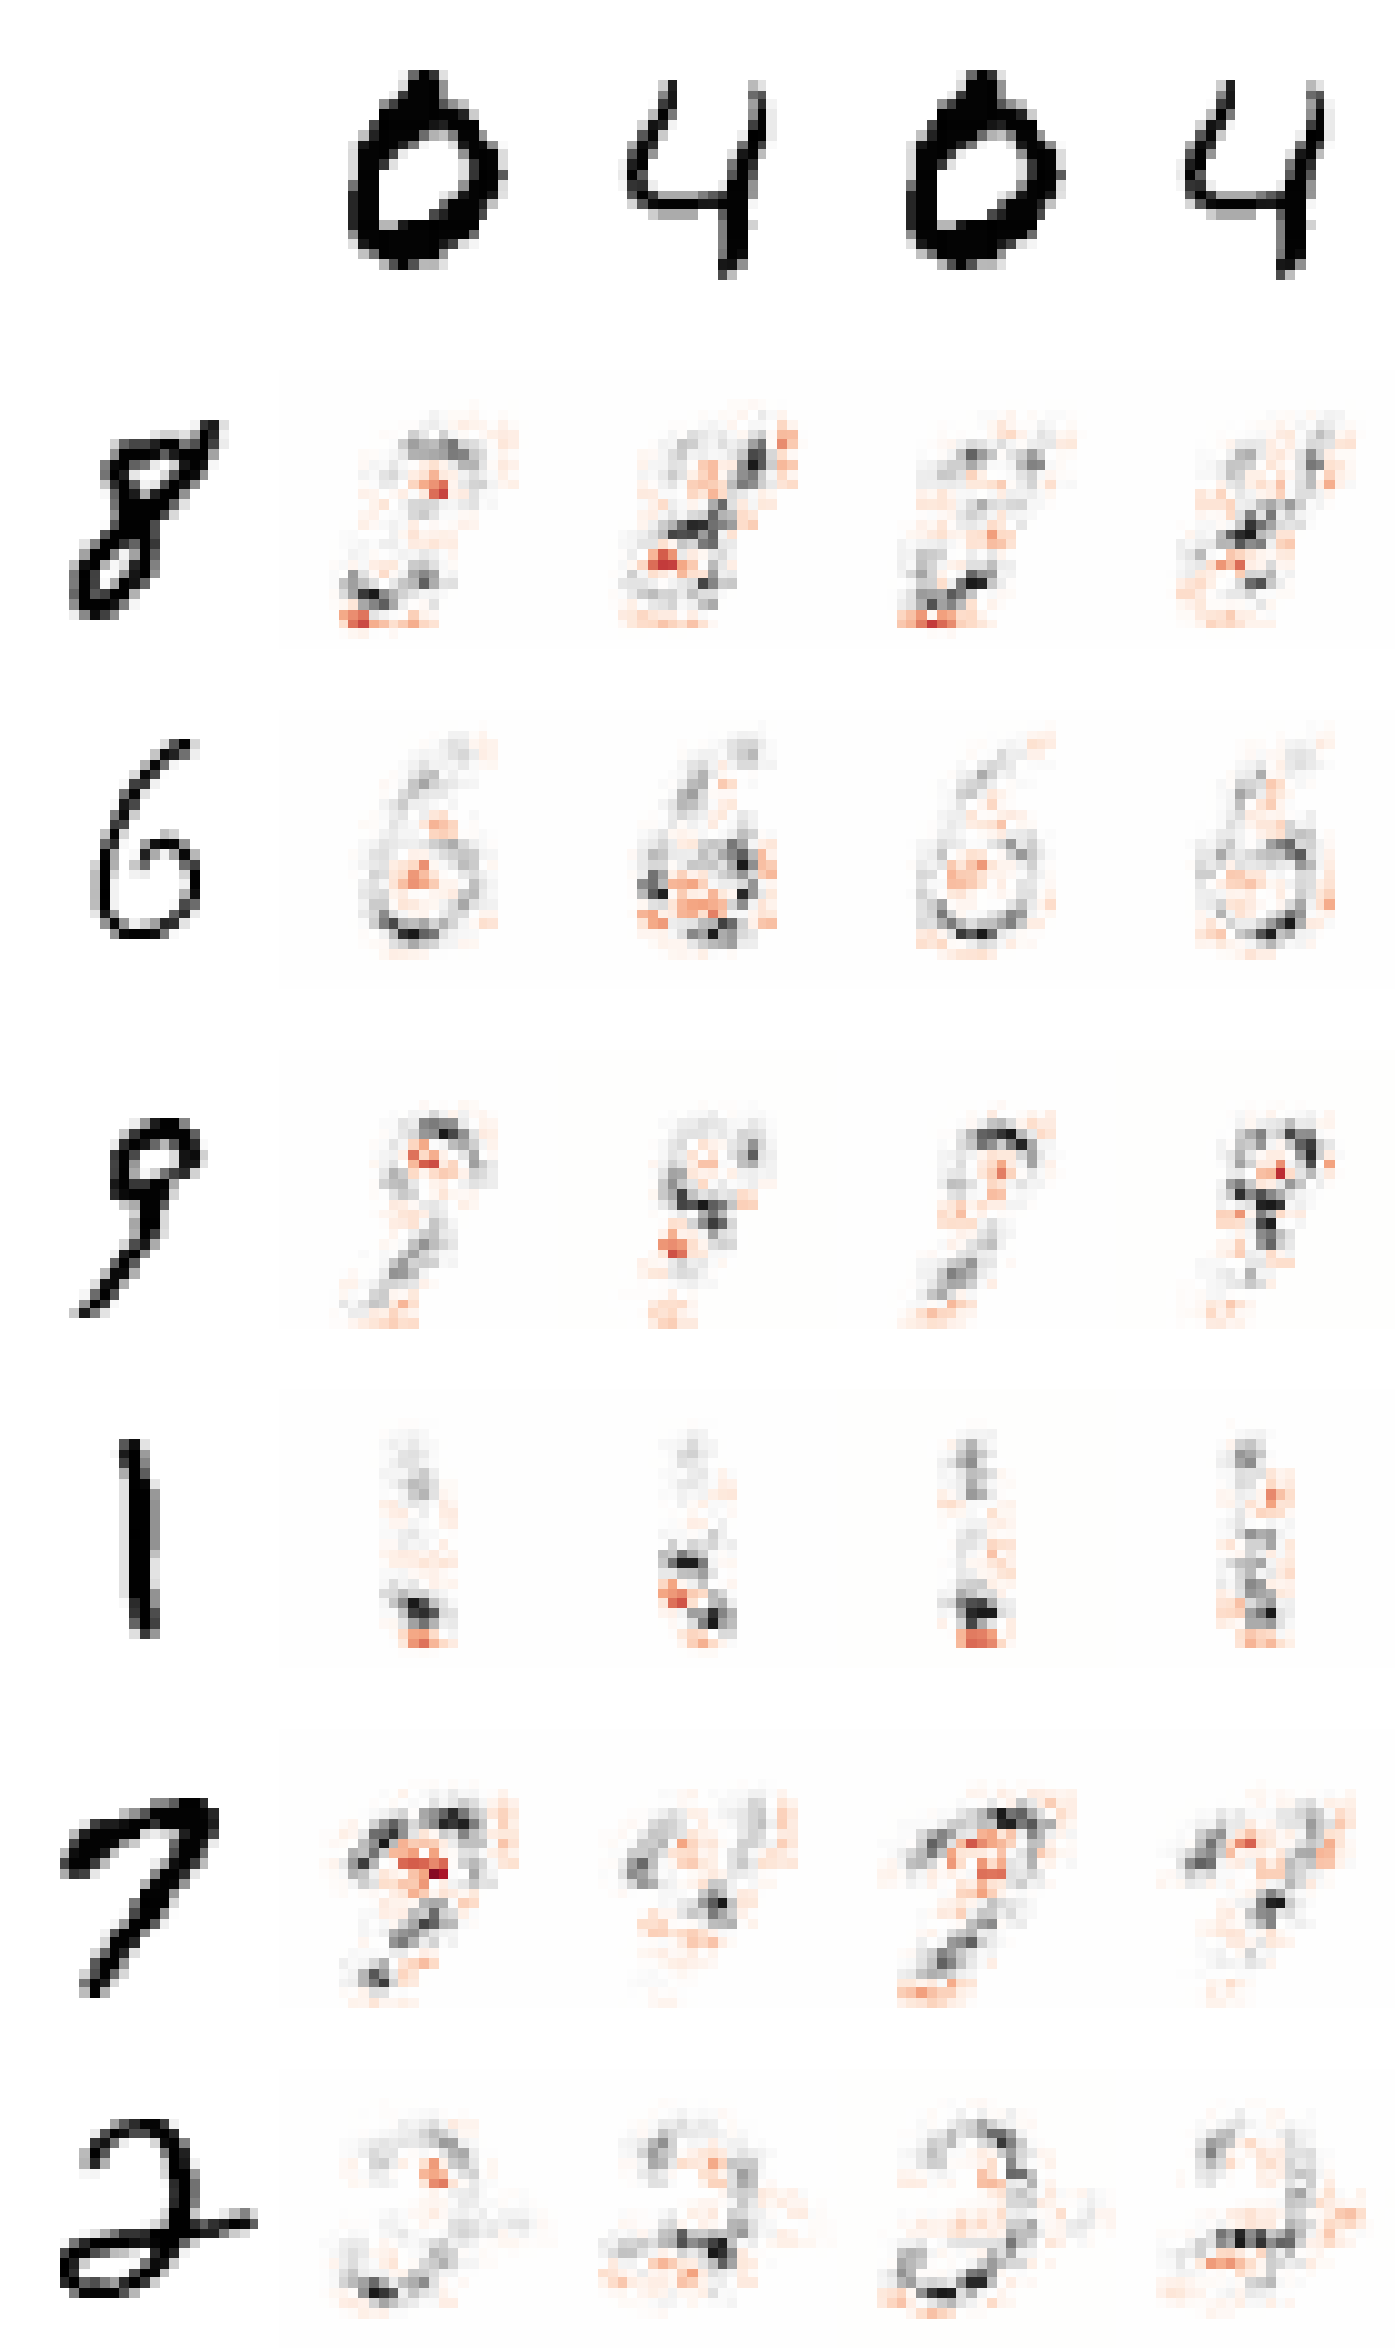
\includegraphics[width=0.35\textwidth]{c4a_figures/grid.pdf}};
    \begin{scope}[x={(image.south east)},y={(image.north west)}]
        %\draw[red,ultra thick,rounded corners] (0.48,0.80) rectangle (0.55,0.95);
        % \draw [-latex, ultra thick, red] (note) to[out=0, in=-120] (0.48,0.80);
        % \draw [-stealth, line width=5pt, cyan] (water) -- ++(0.4,0.0);
    \end{scope}
\end{scope}
\end{tikzpicture}
\begin{subfigure}{0.47\textwidth}
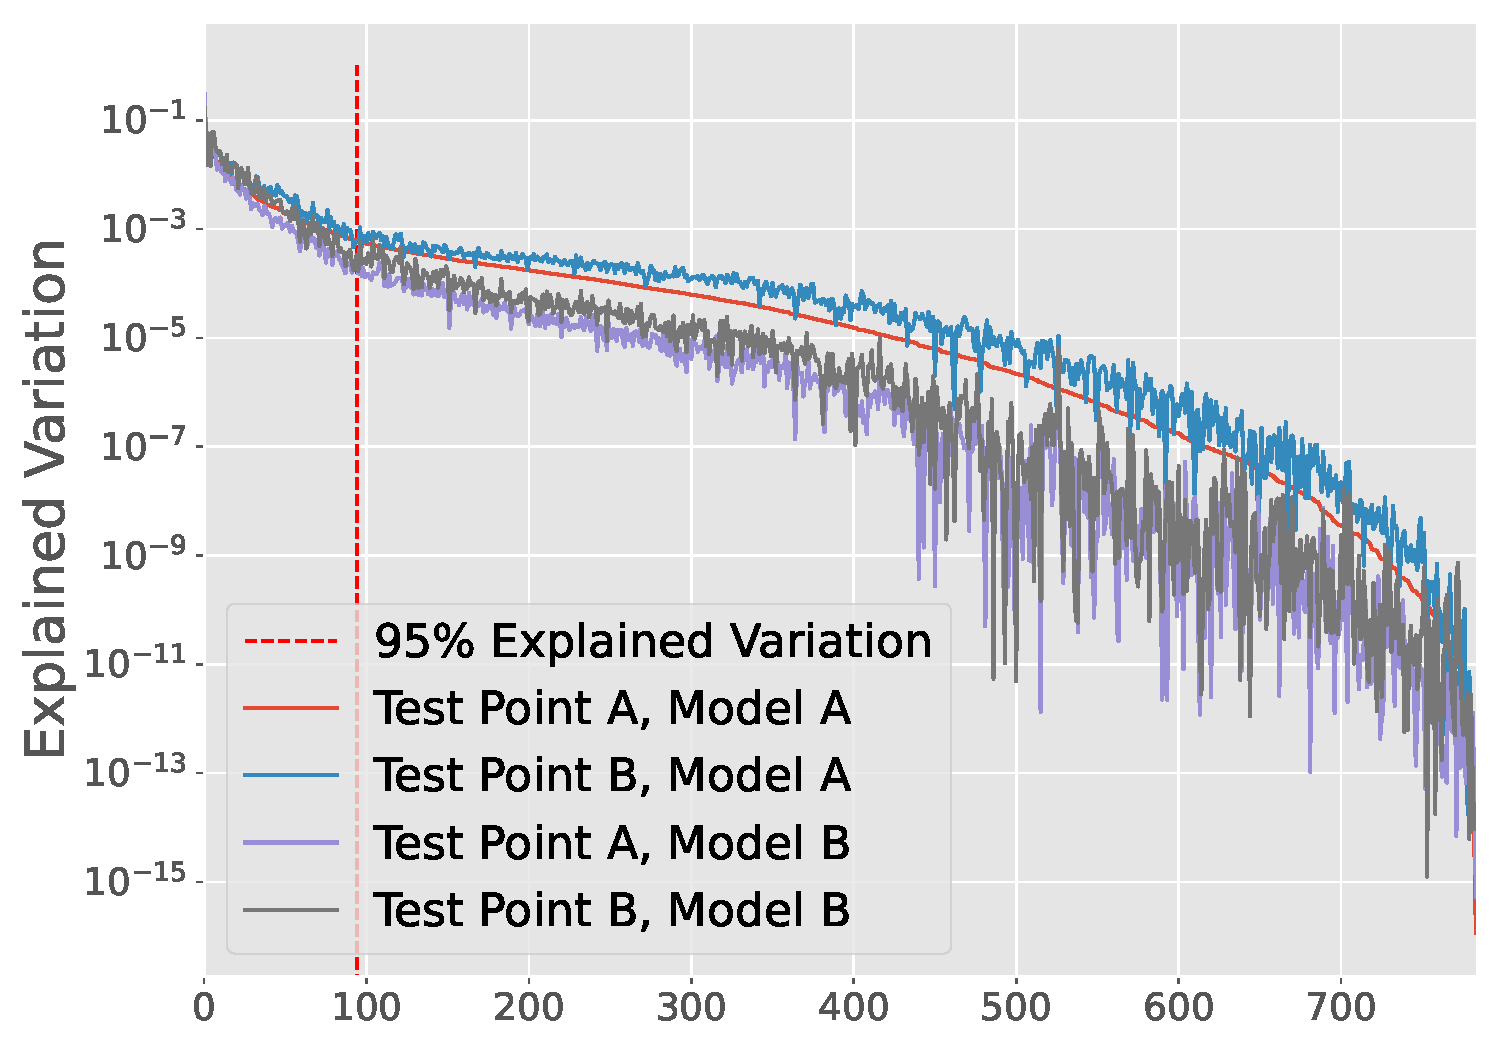
\includegraphics[width=\textwidth]{c4a_figures/related_spectra.pdf}
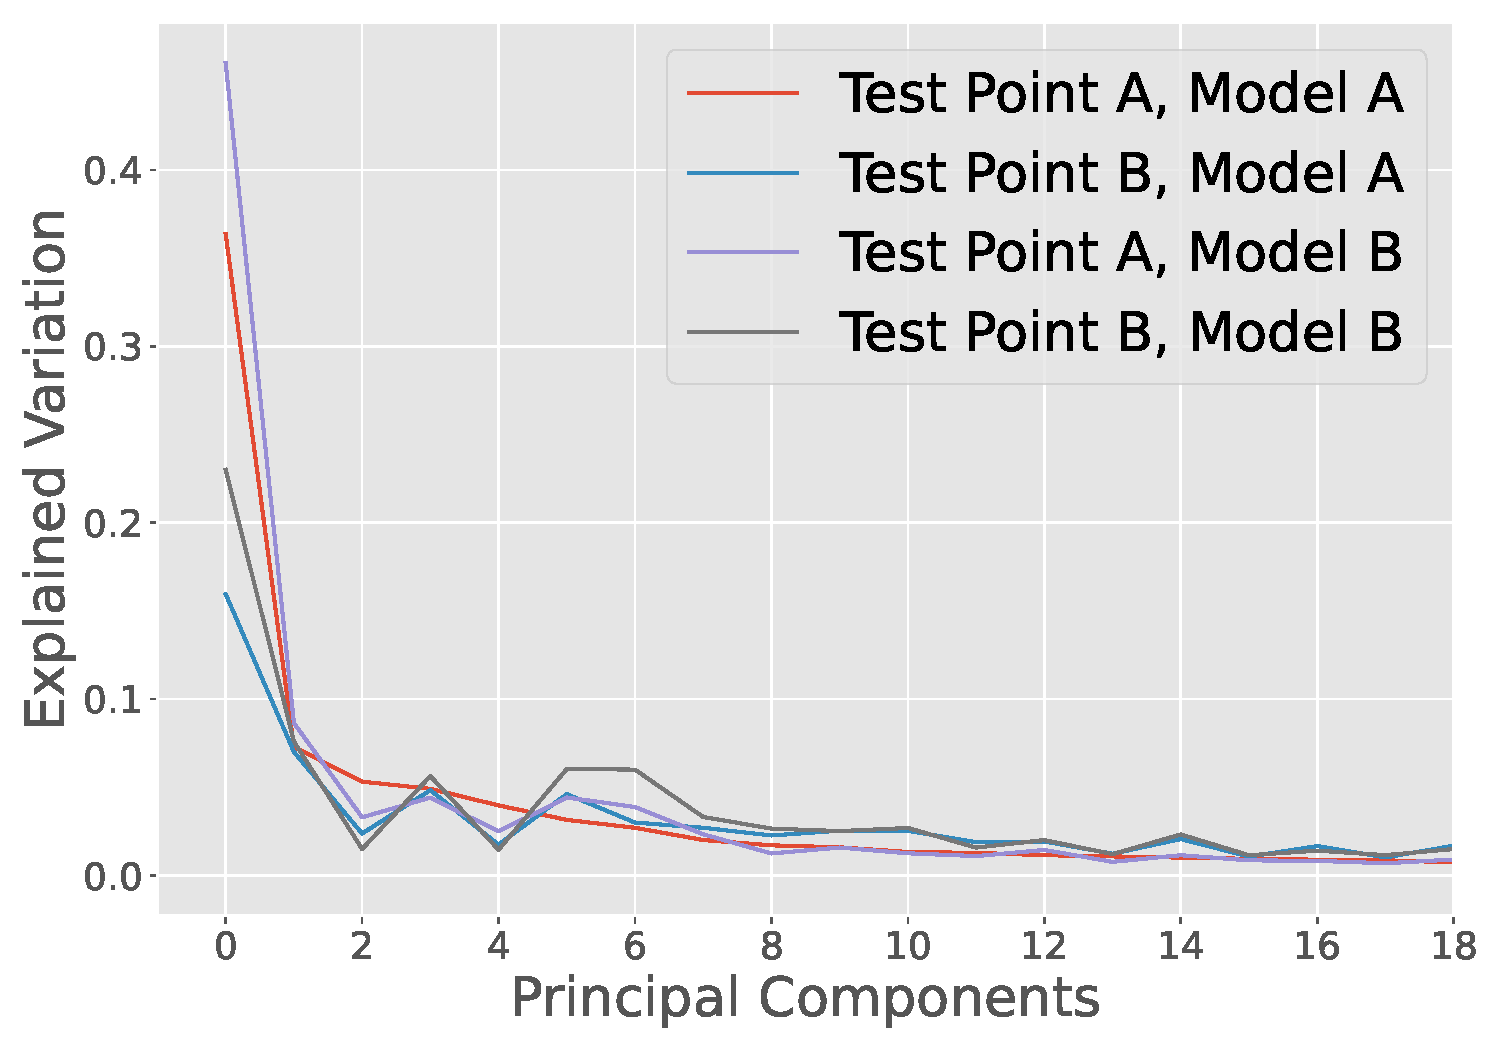
\includegraphics[width=\textwidth]{c4a_figures/related_spectra_narrow_view.pdf}
\end{subfigure}
%\framebox[4.0in]{$\;$}
% \fbox{\rule[-.5cm]{0cm}{4cm} \rule[-.5cm]{4cm}{0cm}}
\end{center}
\caption{Left: Visualization of training point input gradients on test points compared between two models. Positive contribution (black) and negative contribution (red) of each training datum to the prediction for each test point. Elements in the grid are $\nabla_{x_\text{train}}f(x_\text{test}, \theta_\text{trained})$. Right: By taking these individual gradient contributions for a test point and computing the SVD across the training, the significant modes of variation in the input space can be measured (sigma squared). Top is log scale of the full spectrum, bottom shows the first 10 components. Note that this decomposition selects similar, but not identical, modes of variation across test points and even across different models. Components in SVD plots are sorted using Test Point A on Model A.}
\label{fig:trans}
\end{figure}

In addition, we can see that comparison of loss gradients is unnecessary, which allows testing on data without ground truth labels. 
For most applications, the SVD of the parameter gradients over all of the training steps and batches can be pre-computed and compared with test points as needed, although as we can see from this body of work, many simplifying assumptions can be made which will preserve the essential bases needed for performance, but still drastically reduce computational cost. Bottom line: It is not necessarily sufficient to pick a basis that spans a target subspace and then truncate based on its variations. The variations must be accurately measured with correct scaling and, as we can see from the gEPK, implicitly depends on \emph{all} parameter states of the model during training. 


% It is natural to make a variety of simplifying assumptions, e.g. only using a few parameter states, or only the final parameter state as in most of the methods above, to only use a subset of the parameters for the last layer, or to use only a subset of the training data  This simplifying assumption will work when the error vectors and samples are unbiased, but may be leaving meat on the bone by lacking a better measurement of variation 
% is constant, we can consider that 
% The cutting-edge of out-of-distribution detection has come to be occupied by many methods based on gradients. We will examine several of these methods under the lens of our exact representation theorem and its natural decompositions

% Suppose that for the entire training data set $X_{tr}$, we compute 
% \begin{align}
%     \nabla_\theta f(X_{tr}, \theta_{tr}) &= \nabla_\theta f(X_{tr}, \theta_0) + \sum_i \sum_s \int_0^1 \nabla_\theta \dfrac{dL(\hat y_i, y_i)}{d\hat y_i} \langle \varphi_{s,t}(X_{tr}), \varphi_{s,0}(x_i)\rangle + \\
%     &\dfrac{dL(\hat y_i, y_i)}{d\hat y_i} \left( \langle \nabla_\theta \varphi_{s,t}(X_{tr}), \varphi_{s,0}(x_i)\rangle + \langle \varphi_{s,t}(X_{tr}), \nabla_\theta \varphi_{s,0}(x_i)\rangle\right) dt
% \end{align}

% We note that since both $G_{tr, tr} = \nabla_\theta f(X_{tr}, \theta_{tr})$ and $G_{tr, 0} = \nabla_\theta f(X_{tr}, \theta_{0})$ are easily computable, we can remove the latter from the former to estimate the much more complicated summation term. These gradients give us a useful basis in the tangent space for our space of weights $W$. Indeed we can compute the singular value decomposition (SVD): $G_{tr, tr} = U\Sigma V^H$, for which $V^H$ forms a basis for all variation in parameter gradients among training data for the model. We can easily compute the parameter gradients for arbitrary test points $X_{te}$ as $G_{tr, te} = \nabla_\theta f(X_{te}, \theta_{tr})$. Up to a constant scaling factor, we can compute the variation of these test points $X_{te}$ explained by our principal components by element-wise squaring a matrix product $(G_{tr, te} \cdot V)^2$. This allows comparison of the variation of this vector with the primary modes of variation within the image of the training data within the tangent space on weights. 

% A natural question is then to determine whether a set of data has modes of variation which on balance are within the span of these primary modes of variation or not. This can be accomplished by combining projection and norm: $G_{tr, te} V V^H$ to measure the linear variation of test data which lies in the parameter tangent subspace space corresponding with 99\% of the variation from the training data versus not. Another comparison can be made distributionally, examining the spectrum of variation of test points against the spectrum of variation of the training data in the corresponding parameter tangent subspace. 
\section{Signal Manifold Dimension Estimated with Training Input Gradients}



There has been significant interest in quantifying the intrinsic dimension of data \citet{Levina_Bickel_2004,  talwalker2008, ceruti2012, gong2019, Zheng_He_Qiu_Wipf_2022}.
Many such techniques are used to estimate the dimension of intrinsic data manifolds, but do not provide a means to define the manifold itself.
Using the gEPK, it is possible to measure the dimension of signal manifolds observed by the model, and view the exact basis that form the signal manifold around each point.
It is important to note that the gEPK gradient subspaces do not measure the intrinsic dimension of the data. 
Rather, they reflect the dimension of the signal manifold observed by a particular model.
Models which have better representations of data will have a signal manifold more similar to the intrinsic data manifold.
% Additionally, it becomes possible to follow the exact observed manifold in input space.

% % This discussion leans on prior work separating the data manifold from the signal manifold.
% \citet{srinivas2023} define a mask \textbf{m} for every point in input space \textbf{x} such that all information required for classification using a Bayes optimal classifier is contained in $\textbf{x}  \textbf{m}(\textbf{x})$.
% That is to say, the given mask removes all noise from the input.
% This naturally leads also to a definition for the noise manifold, which contains all information not relevant to classification $\textbf{x}  (1-\textbf{m}(\textbf{x}))$. 
% This allows the separation of signal and noise gradients for a given test point.
% % \begin{equation}
% %     \nabla_x p(\textbf{x}|y) = \nabla_x p(\textbf{x}|y) \textbf{m}(\textbf{x}) + \nabla_x p(\textbf{x}|y) (1-\textbf{m}(\textbf{x}))
% % \end{equation}
% The discovery of this mask is difficult in practice.
% Instead of discovering a mask for each test point, it is possible to decompose a test point prediction into the significant training variations that influenced it.


In order to understand the subspace on which a model is sensitive to variation, we may take gradients decomposed into each of the training data. Take, for example, a model, $f(x, \theta)$, which satisfies the necessary conditions for expression as:
\begin{align}
    f(x, \theta_\text{trained}) &= f(x, \theta_0(0)) + \sum_i \sum_s \int_0^1 \varphi_{s,t}(x) \dfrac{dL(x_i, y_i)}{df(x_i, \theta_s(0))} \varphi_{s, 0}(x_i) dt\\
    \varphi_{s,t}(x) &= \nabla_\theta f(x, \theta_s(t))
\end{align}
And $\theta_s(t)$ are the parameters of $f$ for training step $s$ and time $t$ so that $\sum_s \int_0^1 \theta_s(t) dt$ integrates the entire training path taken by the model during training. Given a test point $x$, we can evaluate its subspace by taking, for each $x_i$:
\begin{align}
    \dfrac{df(x, \theta_\text{trained})}{dx_j} &= \dfrac{df(x, \theta_0(0))}{dx_j} + \sum_i \sum_s \int_0^1 \dfrac{d\left(\varphi_{s,t}(x) \dfrac{dL(x_i, y_i)}{df(x_i, \theta_s(0))} \varphi_{s, 0}(x_i)\right)}{dx_j} dt\\
    &= 0 + \sum_i \sum_s \int_0^1 \varphi_{s,t}(x) \dfrac{d\left(\dfrac{dL(x_i, y_i)}{df(x_i, \theta_s(0))} \varphi_{s, 0}(x_i)\right)}{dx_j} dt \\
    &= \sum_i \sum_s \int_0^1 \varphi_{s,t}(x)dt \left(\dfrac{d^2L(x_i, y_i)}{df(x_i, \theta_s(0)) dx_j} \varphi_{s, 0}(x_i) + \dfrac{dL(x_i, y_i)}{df(x_i, \theta_s(0))} \dfrac{d\varphi_{s, 0}(x_i)}{dx_j}\right) 
\end{align}
We can see that these gradients will be zero except when $i = j$, thus we may summarize these gradients as a matrix (tensor in the multi-class case), $G$, with 
\begin{align}
    G_j = \sum_s \int_0^1 \varphi_{s,t}(x)dt \left(\dfrac{d^2L(x_i, y_i)}{df(x_i, \theta_s(0)) dx_j} \varphi_{s, 0}(x_i) + \dfrac{dL(x_i, y_i)}{df(x_i, \theta_s(0))} \dfrac{d\varphi_{s, 0}(x_i)}{dx_j}\right)
    \label{eq:input_decomp}
\end{align}
While written in this form, it appears we must keep second-order derivatives, however we note that the inner product with $\phi_{s,t}(x)$ eliminates these extra dimensions, so that clever implementation still only requires storage of vectors (low rank matrices in the multi-class case). 

The rank of $G$ represents the dimension of the subspace on which the model perceives a test point, $x$, to live, and we can get more detailed information about the variation explained by the span of this matrix by taking its singular value decomposition (SVD). We can exactly measure the variation explained by each orthogonal component of the $\text{span}(G)$ with respect to the given test point $x$. $G(x)$ can be defined as a map from $x$ to the subspace perceived by the model around $x$. Any local variations in the input space which do not lie on the subspace spanned by $G(x)$ can not be perceived by the model, and will have no effect on the models output.

On MNIST, $G(x)$ creates a matrix which is of size $60000 \times 784$ (training points $\times$ input dimension).
This matrix represents the exact measure of each training points contribution towards a given test prediction.
Of note is that in practice this matrix is full rank on the input space as seen in Figure \ref{fig:trans}.
This is despite MNIST having significantly less degrees of variation than its total input size (many pixels in input space are always 0).
Figure \ref{fig:cdf} demonstrates that accounting for 95\% of the variation requires only 94 (12\%) of the 784 components on average.
Similarly, on CIFAR accounting for 95\% of explained variation requires 1064 (34\%) of the 3096 components.
It is likely that different training techniques will provide significantly different signal manifolds and consequently different numbers of components.
Examining these effects may lead to deeper understanding of optimization techniques.

\begin{figure}[t]
    \centering
    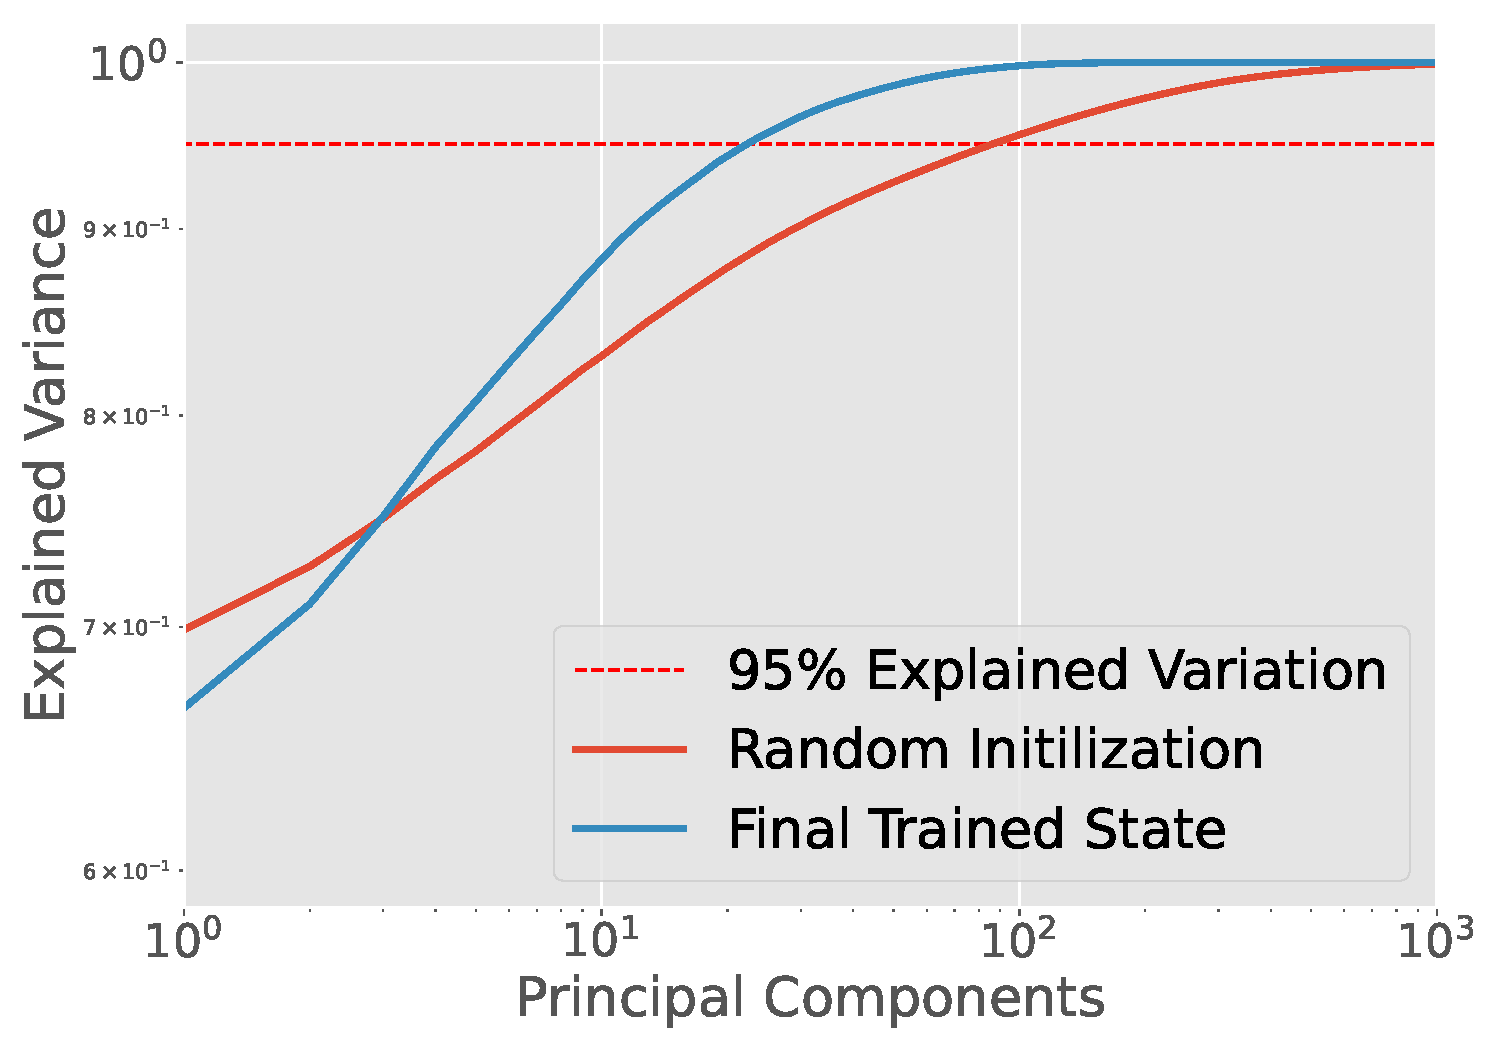
\includegraphics[width=.45\textwidth]{c4a_figures/dimension_change_weightspace.pdf}
    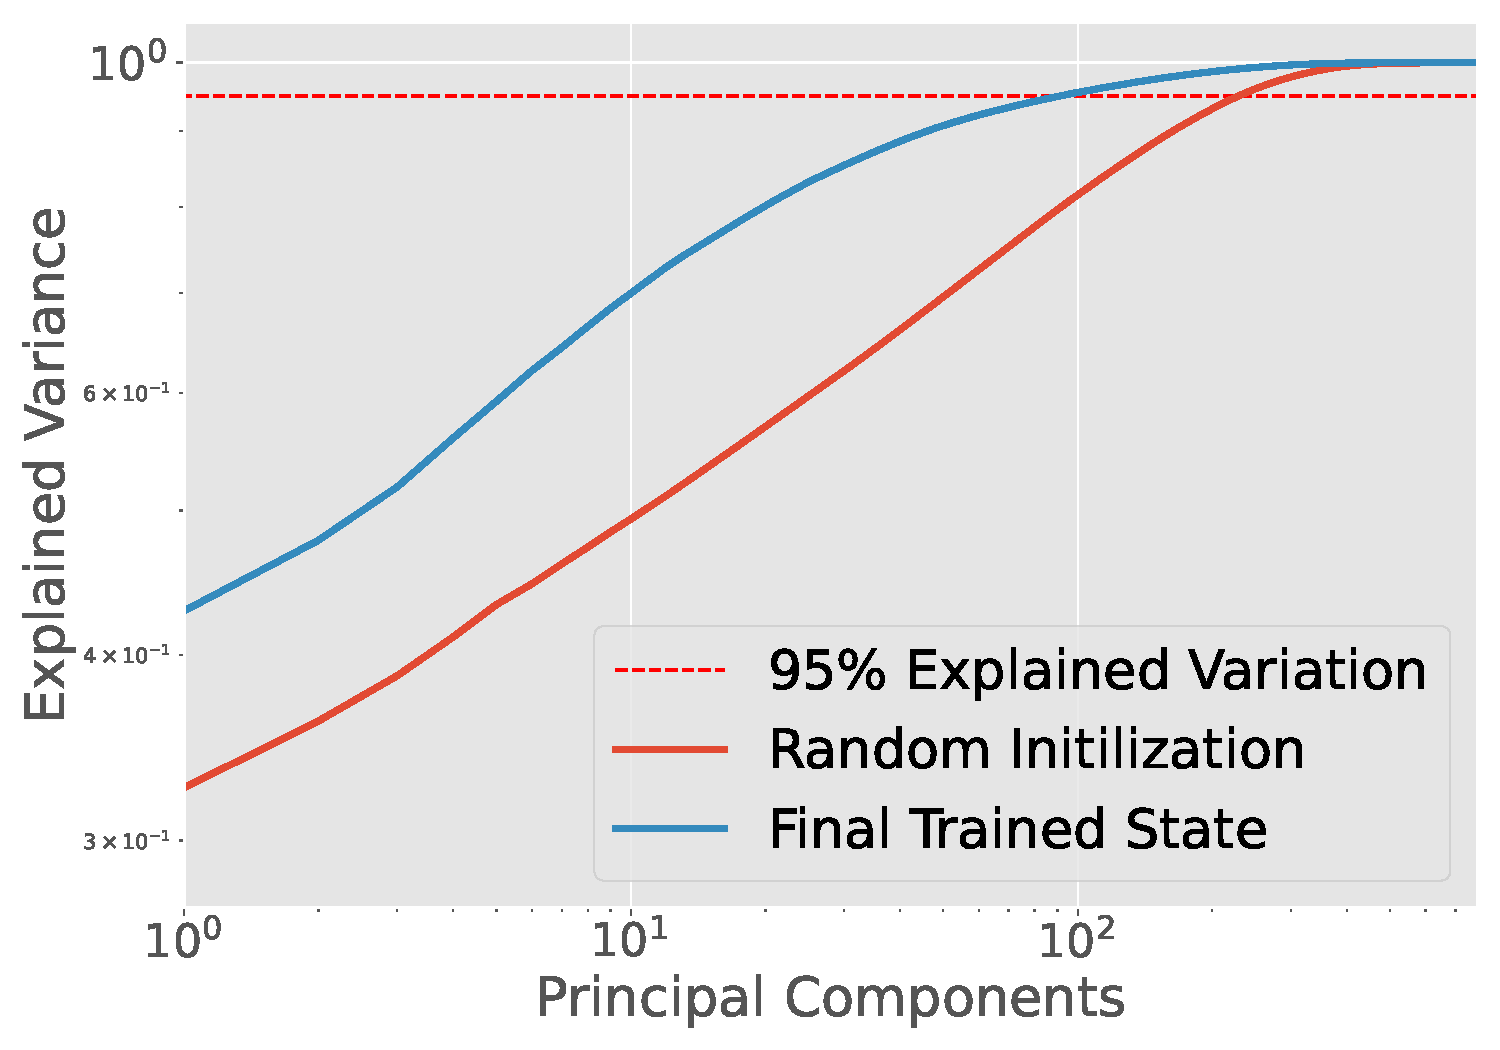
\includegraphics[width=.45\textwidth]{c4a_figures/dimension_change.pdf}
    \caption{Differences between observing gradients in input space vs. weight space. Left: CDF of explained variation parameter space. Right: CDF of explained variation input space. Red solid line indicates a model at random initialization while the blue solid line represents the fully trained state. From random initialization, the number of principal components required to achieve 95\% explained variation decreases in both cases. Note that at random initialization, the weight space gradients already have only a few directions accounting for significant variation. Disentangling the data dimension using weight space gradients is less effective than doing so in input space \citep{shamir2021dimpled}.}
    \label{fig:compare}
\end{figure}

% Exploring the dimension of data using 

% The EPK formulation allows for calculation of test point sensitivity to the training set $\frac{\partial f(x, \theta_{trained})}{\partial x_{train}}$.
% The dimension of a models signal manifold can be estimated by observing the SVD of this .
% Prior to the introduction of the EPK, it was not possible to measure this quantity.

% By observing the full set of input gradients on the training set centered at a given test point, it is possible to construct a complete list of all data variations which influenced a test point prediction.
% This basis is over determined, and it is likely that there are many redundant degrees of variation.
% By taking the Singular Value Decomposition of these it becomes possible to measure the significant modes of input variation the model considered during training.


We can also examine this subspace with less granularity by taking the parameter gradients for each training point from its trained state. This involves using each training point as a test point. 
\begin{align}
    \dfrac{df(x_j, \theta_\text{trained})}{dx_j} &= \dfrac{df(x_j, \theta_0(0))}{dx_j} + \sum_i \sum_s \int_0^1 \dfrac{d\left(\varphi_{s,t}(x_j) \dfrac{dL(x_i, y_i)}{df(x_i, \theta_s(0))} \varphi_{s, 0}(x_i)\right)}{dx_j} dt
\end{align}
The left hand side is computable without path-decomposition and so can be computed for each training datum to create a gradient matrix, $H_{\theta_\text{trained}}$. Another term, $\dfrac{df(x_j, \theta_0(0))}{dx_j}$ is also easily computable, yielding another matrix $H_{\theta_0}$. By comparing the rank and span of $H_{\theta_\text{trained}}$ and $H_{\theta_0}$ we can understand to what extent the model's spatial representation of the data is due to the initial parameter selection and how much is due to the training path. Also, $H_{\theta_\text{trained}}$ provides sample of gradients across all training data, which in some sense must be spanned by the model's implicit subspace basis. Despite missing the granular subspace information, the rank of this gradient matrix and its explained variation computed using SVD should be related to the model's implicit subspace rank. 
It should be noted that while there is a direct relationship between a models variations in input space and weight space, Figure \ref{fig:compare} shows that this mapping changes greatly from the beginning to end of training and that this spectrum starts out wide (high dimensional) for $\theta_0$ and much more focused (low dimensional) for $\theta_T$. 


%
% \subsection{Few-Step Hindsight Learning}

% (I was thinking this goes in a new subsection in the Experiments section)
% \begin{figure}
%     \centering
%     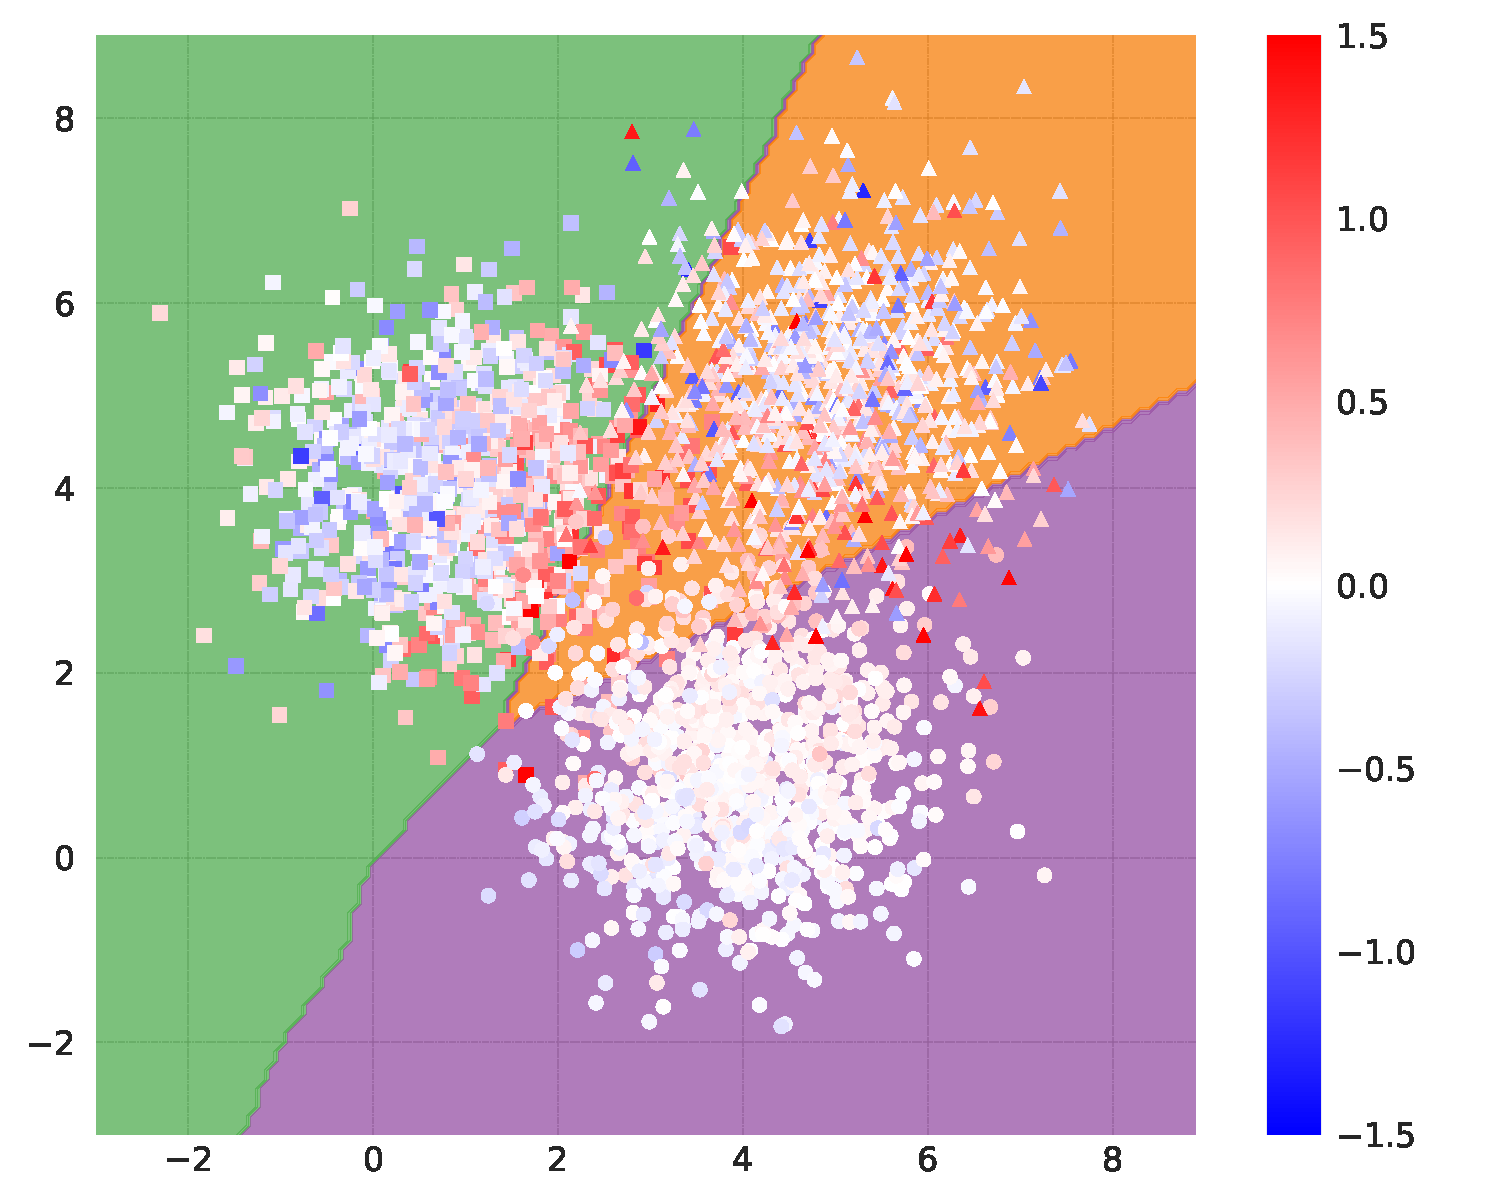
\includegraphics[width=0.4\linewidth]{c4a_figures/adaptive_output_a.pdf}
%     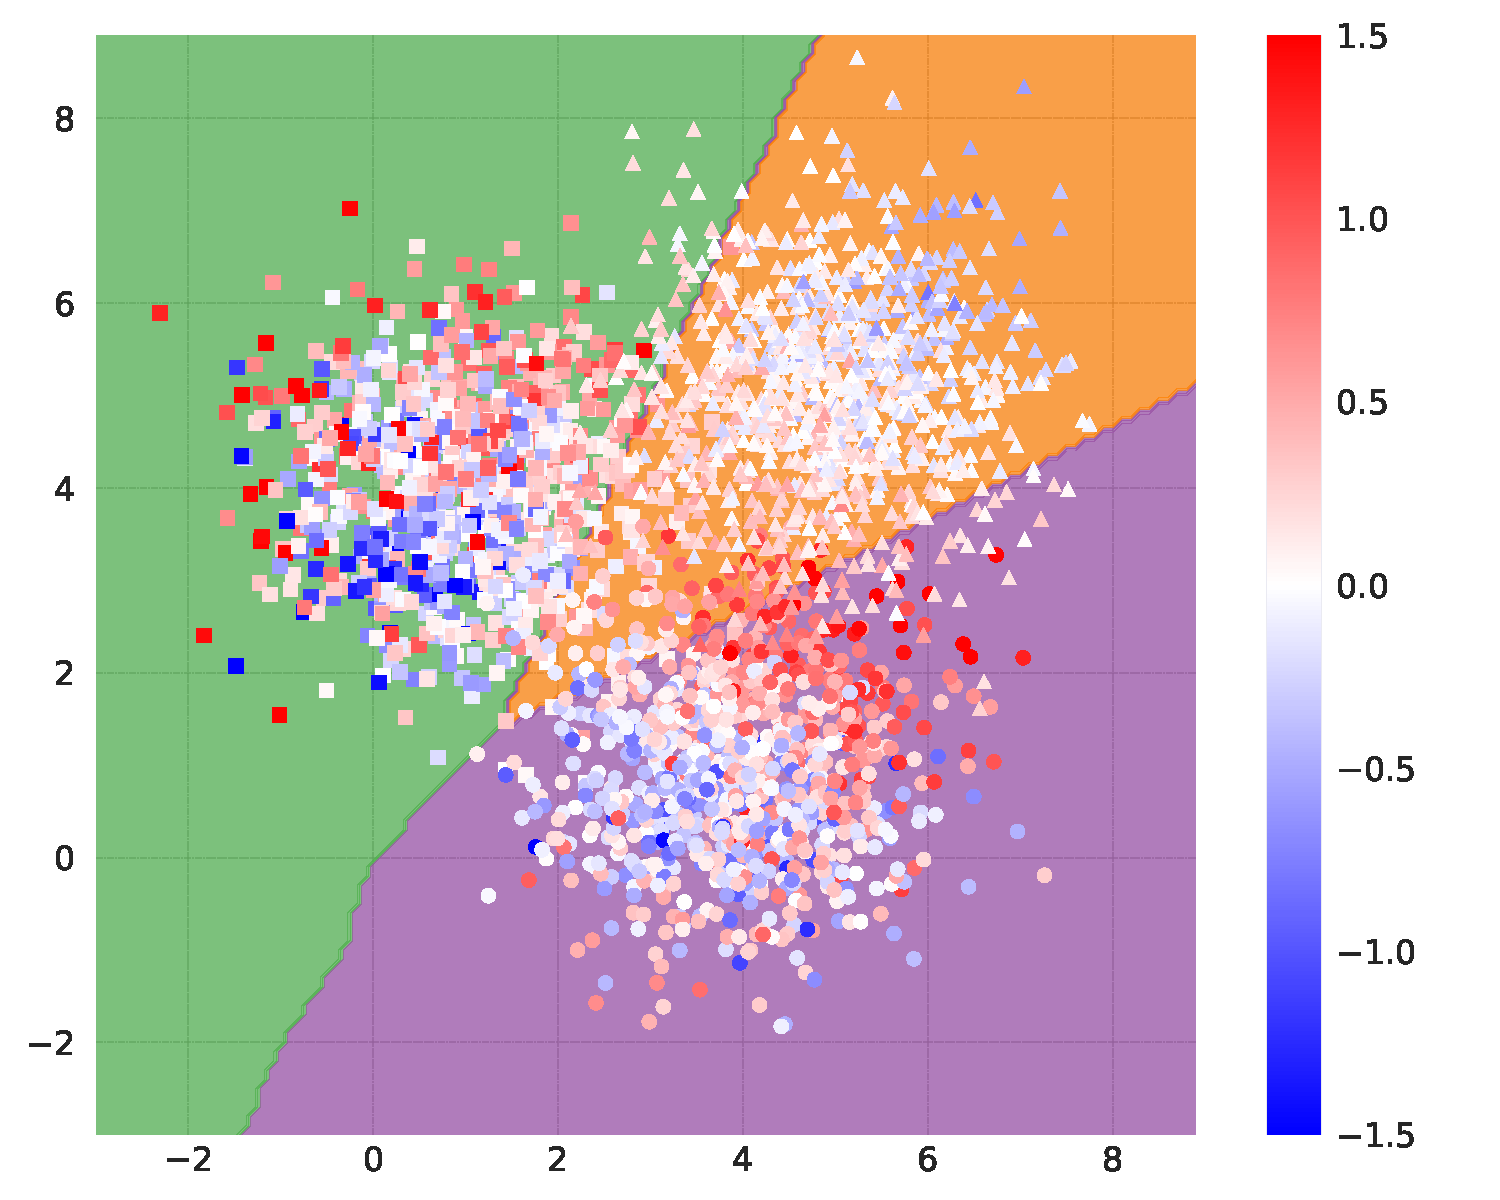
\includegraphics[width=0.4\linewidth]{c4a_figures/adaptive_output_b.pdf}
%     \caption{Caption}
%     \label{fig:enter-label}
% \end{figure}

% Computing this full kernel representation is expensive and a substantial part of this computational cost is from the need to store and load large numbers of parameter states for the model. Therefore we could achieve a substantial decrease in computational expense by reducing the number of steps needed for training. We will use hindsight to achieve this. Given the parameters $\theta_{T}$ from a fully trained model $f(x; \theta_{T})$, and the initial parameters $\theta_0$ for that model we will attempt to reach $\theta_{T}$ in as few steps as possible. In order to remain within the span of the parameter gradients on our training, we will require that each step be constructed from a weighted sum of initial training gradients: 
% \begin{align}
%     \theta_1 = \theta_0 + \sum_i \varepsilon \nabla_\theta f(x; \theta_0)
% \end{align}
% under this constraint we will select $\varepsilon$ as 
% \begin{align}
%     \{\varepsilon\} &= \text{argmin}_{\{\varepsilon\}} \| \theta_T - \theta_0 - \sum_i \varepsilon \nabla_\theta f(x; \theta_0) \|_2
% \end{align}
% We can compute this with least squares with 
% \begin{align}
%     A &= \nabla_\theta f(X_{\text{Train}}; \theta_0)\\
%     b &= \theta_0 - \theta_T\\
%     A\varepsilon &= b\\
%     A &= U\Sigma V^H\\
%     \varepsilon' &= (V \Sigma^+U^H)b \\
%     \Sigma^+_i &= \begin{cases} \Sigm\varepsilon^{-1} & \text{if} \sigm\varepsilon \neq 0, \\ 0 & \text{if} \Sigm\varepsilon = 0. \end{cases}
% \end{align}
% Conveniently, since we are only adding a constant scalar to each of our training gradients, our exact representation does not change by much
% \begin{align}
%     f(x; \theta_{1}) &= f(x; \theta_0) + \sum_i a'_i \int_0^1 \varphi_{0,t}(x) \dfrac{dL(x_i, y_i)}{df(x_i; \theta_0(0))} \varphi_{0, 0}(x_i) dt 
% \end{align}

% Implementing this experimentally, we discovered that the span of the training gradients for the initial training parameters $\theta_0$ $\theta_0$ did not cover the vector $\theta_F - \theta_0$. This appears to be due to the relatively small number of principal components which explain 99\% of the varaiation in the training vectors for $\theta_0$. An extra step or two are required, following the same procedure, in order to achieve a clear match with the final weight. 

% \begin{figure}[ht]
% \begin{center}
% 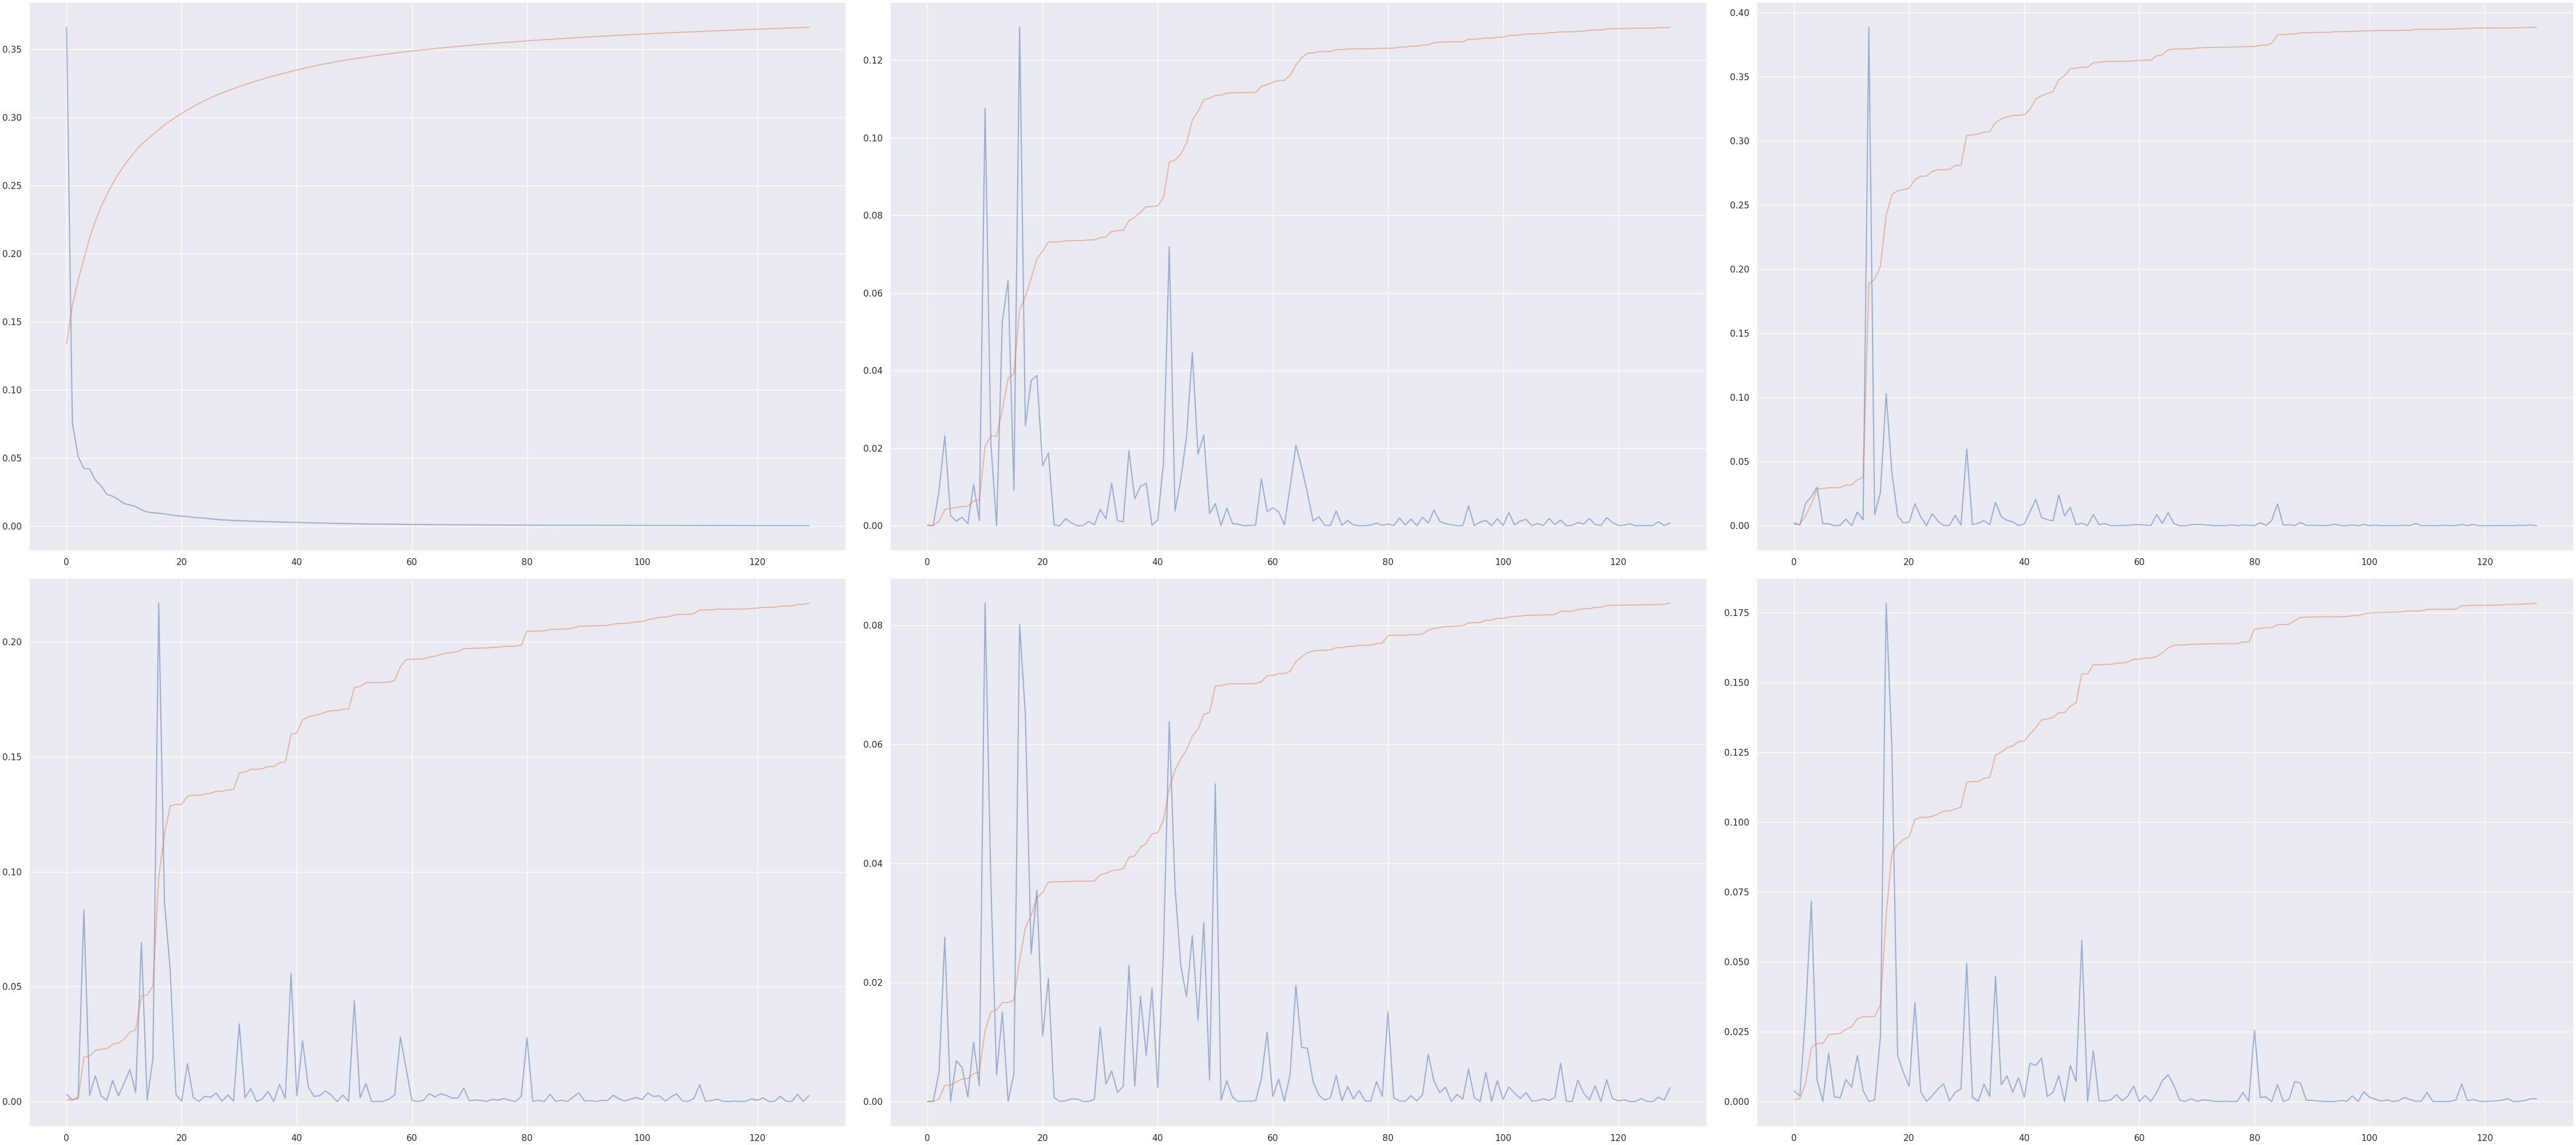
\includegraphics[width=0.8\textwidth, trim={0 0 40cm 0},clip]{c4a_figures/mnist_ntk_input_spectrum-130.png}
% %\framebox[4.0in]{$\;$}
% % \fbox{\rule[-.5cm]{0cm}{4cm} \rule[-.5cm]{4cm}{0cm}}
% \end{center}
% \caption{Input gradient projection onto principal components for upper-left test image. Rows are different final trained states of the model. Columns correspond to different test images. This plot has been truncated at 120 out of 784 components for visibility. The order of components determined by the top left example. Note that the principal components visible to the model are aligned in the input space, even with different weight states.}
% \label{fig:trans}
% \end{figure}

One interesting property of using input gradients for training data decomposed according to Eq.~\ref{eq:input_decomp} is the ability to compare input gradients across models with different initial parameters and even different architectures.
Figure \ref{fig:trans} demonstrates that two models with different random initializations which have been trained on the same dataset have a signal manifold which shares many components.
This is a known result that has been explored in deep learning through properties of adversarial transferability~\citet{szegedy2013intriguing}.
This demonstrates that the gEPK is capable of measuring the degree to which two models rely on the same features directly.
This discovery may lead to the construction of models which are provably robust against transfer attacks.

% \subsection{Bound Signal Manifold Dimension with Kernel Parameter Decomposition}
% \subsubsection{Signal Manifold Dimension Drops During Training}
% \subsubsection{Few-Step Learning Reveals difference in Early versus Late Training Contributions}
% \subsubsection{Signal Manifold Dimension Match Between Both Decompositions }
% \subsection{Expose OOD Samples with Kernel Parameter Decomposition}


\section{Conclusion}

This paper presented a general exact path kernel representation for neural networks with a natural decomposition that connects existing out-of-distribution detection methods to a theoretical baseline. This same representation reveals additional connections to dimension estimation and adversarial transferability. These connections are demonstrated with experimental results on computer vision datasets. The key insights provided by this decomposition in this work are that model predictions implicitly depend on the parameter tangent space on its training data and that this dependence enables decomposition relative to a single test point by either parameter gradients, or training input gradients. This allows users to connect how neural networks learn at training time with how each training point influences the final decisions of a network.

This method has many theoretical connections to continuing work in this area including better understanding of how models depend on implicit prior distributions following (e.g.~\citet{nagler2023}), supporting more robust statistical learning under distribution shifts (e.g. \citet{Simchowitz2023}), and supporting more robust learning by connecting with a growing body of work applying gradients to OOD detection and more generally by connecting to recent results by~\citet{desilva2023} which indicate that understanding OOD data can make models more general. 

\newpage

% \subsubsection*{Author Contributions}


% \subsubsection*{Acknowledgments}

%\bibliography{iclr2024_conference}
%\bibliographystyle{iclr2024_conference}
